\documentclass[a4paper,12pt, centered]{bookest}
\usepackage[ukrainian,english]{babel}
\usepackage{ucs}
\usepackage[utf8]{inputenc}
\usepackage[T2A]{fontenc}
\usepackage{amsmath}
\usepackage{amsfonts}
\usepackage{scalerel}
\usepackage{amsthm}
\usepackage{mdframed} 
\usepackage{xcolor}
\usepackage{xparse}
\usepackage{amssymb}
\usepackage{tikz} 
\usepackage{afterpage}
\usepackage{wrapfig}
\usepackage[makeroom]{cancel}
\usepackage{booktabs,caption}          
\usepackage[flushleft]{threeparttable}
\definecolor{black}{cmyk}{.30,0,0,.67} 
\title{Дискретна математика 2\\ \small (Discrete mathematics)
}

\date{\today}
\newtheorem{theorem}{Theorem}[section]
\newtheorem*{theorem*}{Theorem}
\newtheorem{corollary}{Corollary}[theorem]
\newtheorem{lemma}[theorem]{Lemma}
\newtheorem{definition}{Definition}[section]
\newtheorem{property}{Property}
\newtheorem*{property*}{Property}
\newtheorem*{prop*}{Proposition}
\newtheorem{cons}{Consequence}
\newtheorem*{cons*}{Consequence}
\newtheorem*{fact*}{Fact}
\newtheorem*{remark*}{\emph{Remark}}
\newcommand*\circled[1]{\tikz[baseline=(char.base)]{
            \node[shape=circle,draw,inner sep=2pt] (char) {#1};}}
\DeclareMathOperator{\lcm}{lcm}
\DeclareMathOperator{\ord}{ord}
\DeclareMathOperator{\Aa}{\mathcal{A}}
\DeclareMathOperator{\Mm}{\mathcal{M}}
\DeclareMathOperator{\im}{Im}
\DeclareMathOperator{\blank}{ }
\newcommand\tab[1][1cm]{\hspace*{#1}}
\newcommand\bigbang{\vcenter{\hbox{\resizebox{!}{1.6$\Bigg$}{!}}}}
\newmdenv[   linecolor=black,
  topline=false,
  bottomline=false,
  rightline=false,
  skipabove=\topsep,
  skipbelow=\topsep
]{leftrule}

\NewDocumentEnvironment{example}{O{\textbf{Example:}}} {\begin{leftrule}\noindent\textcolor{black}{#1}\par}
{\end{leftrule}}
\catcode`@=11
\def\caseswithdelim#1#2{\left#1\,\vcenter{\normalbaselines\m@th
  \ialign{\strut$##\hfil$&\quad##\hfil\crcr#2\crcr}}\right.}\catcode`@=12

\def\bcases#1{\caseswithdelim[{#1}}
\def\vcases#1{\caseswithdelim|{#1}}
\usepackage[titletoc]{appendix}
\begin{document}
\maketitle
\vspace*{\fill}
\begin{flushright}
\emph{*Лекция начинается*}\\
\emph{-Сегодня у нас клуб уопоротых любителей математики.}
\end{flushright}
\let\cleardoublepage\clearpage
\tableofcontents
\newpage
\thispagestyle{empty}
\hspace{0pt}
\vfill
\begin{center}
	\LARGE{\textbf{Основа теорії чисел}}
\end{center}
\begin{center}
	(Fundamentals of Number theory)
\end{center}
\vfill
\hspace{0pt}
\pagebreak
\newpage
\chapter{Лекція 1}
\section{Подільність чисел}
	\begin{enumerate}
		\item[-]властивості натуральних чисел\\
		$\mathbb{N}=\{1,\>2,\>3,\dots\}\\
		\mathbb{N}_0=\{0,\>1,\>2,\>3,\dots\}\\
		\mathbb{Z}=\{-1,\>0,\>1,-2,\>2,\dots\}$
	\end{enumerate}
	\begin{definition}
		$a$ поділяється на $b\>\>-\>\>a\>\vdots\>b$ або  $b$ ділить $a$($b$ є дільником$a$)$\>\>b\>|\>a.$
		$$a\>\vdots\>b\Leftrightarrow\exists k\in\mathbb{Z}:\>\>a=kb$$
	\end{definition}
	\begin{property*}$ $
	\begin{enumerate}
		\item $a\neq 0,\>\>a\>\vdots\>0$
		\item $a\neq 0,\>\>0\>\vdots\>a$
		\item $a\>\vdots\>b,\>b\>\vdots\>c\Rightarrow a\>\vdots\>c$
		\item $a\>\vdots\>1$
		\item $a\>\vdots\>c,\>b\>\vdots\>c\Rightarrow (\alpha a\pm\beta b)\>\vdots\>c$
		\item $a\>\vdots\>b\Leftrightarrow ac\>\vdots\>bc,\>c>0$
	\end{enumerate}		
	\end{property*}
	\begin{theorem}[Euclidean divisiom] 
	$$\forall a,\>b\in\mathbb{Z}\>\>\exists!q,\>r\>:\>q\in\mathbb{Z},\>r\in\mathbb{N}\>\>0\leq r\leq |b|\>\>a=bq+r$$
	\newpage
	\begin{proof}$ $
		\begin{enumerate}
			\item Існування\\
			$bq,\>q\in\mathbb{Z}$ - росте необмежено. $\exists q\>;\>bq\leq a\leq b(q+1),\>r=a-bq.$
			\item Єдиність\\
			Нехай $a=bq+r,\>\>a=bq'+r'\\
			0=b(q-q')+(r-r')\Rightarrow(r-r')\>\vdots\>b,\>-|b|<r-r'<|b|\Rightarrow\\\Rightarrow r-r'=0,\>q=q'.$
		\end{enumerate}
	\end{proof}
	\end{theorem}
	$q=\lfloor\dfrac{a}{b}\rfloor$ - частка.\\
	$r=a+b\cdot\lfloor\dfrac{a}{b}\rfloor$ - остача $=a\mod b$.
\section{Найбільший спільний дільник	}
Найбільший спільний дільник: НСД$(a,\>b)$(українська нотація), $\gcd(a,\>b)$(англійська нотація), $(a,\>b)$(спеціальзована література з теорії чисел). 
	\begin{definition}
		$\gcd(a,\>b)=d:$
		\begin{enumerate}
			\item $a\>\vdots\>d,\>b\>\vdots\>d$
			\item $d\>-\>\max$ додатнє число, яке задовільняє 1.
		\end{enumerate}
	\end{definition}
	\begin{property*}$ $
		\begin{enumerate}
			\item $\gcd(a,\>b)=b\Leftrightarrow a\>\vdots\>b$
			\item $a\neq 0:\>\gcd(a, 0)=a$
			\item $\gcd(a,\>b)$ поділяеться на довільний спільний дільник a та b
			\item $c>0:\>gcd(ac,\>bc)=c\gcd(a,\>b)$ 
			\item $d=\gcd(a,\>b)\Rightarrow \gcd(\dfrac{a}{d},\>\dfrac{b}{d})$
		\end{enumerate}
	\end{property*}
	\newpage
	\begin{lemma}
		$$\gcd(a,\>b)=\gcd(b,\>a-b)$$
	\begin{proof}
		$\\ d=\gcd(a,\>b),\>d'=\gcd(b,\>a-b)\\\textrm{Нехай } d>d'\\a\>\vdots\>d,\>b\>\vdots\>d\Rightarrow(a-b)\>\vdots\>d\Rightarrow d\textrm{ - спільний дільник b та a-b}\Rightarrow d'\>\vdots\>d$ - Упс!\\
		$\textrm{Нехай }d<d'\\ b\>\vdots\>d',\>a-b\Rightarrow b+(a-b)=a\>\vdots\>d'$ - Упс!
	\end{proof}
	\begin{cons*}
		$$a\geq b:\>\>\gcd(a,\>b)=(b,\>a\mod b)$$
		\begin{proof}
			$a=bq+r\\
			\gcd(a,\>b)\underbrace{=\dots=}_{q\textrm{ разів}}\gcd(r,\>b)$
		\end{proof}
	\end{cons*}
	\end{lemma}
\section{Алгоритм Евкліда}
Вхід: $a,\>b\in\mathbb{N}$\\
Вихід: $d=\gcd(a,\>b)$\\\\
$\tab r_0:=a,\>r_1:=b$\\
$\tab r_0=r_1q_1+r_2$\\
$\tab r_1=r_2q_2+r_3$\\
$\tab r_2=r_3q_3+r_4$\\
$\tab\quad\vdots$\\
$\tab r_{n-1}=r_nq_n,\>\>r_n=d$
\begin{proof}
	$r_{i+1}=r_{i}\mod r_{i-1}\\ r_0\geq r_1>r_2>\dots>r_{n}>r_{n+1}=0\\\gcd(a,\>b)-\gcd(r_0,\>r_1)=\gcd(r_1,\>r_2)=\gcd(r_2,\>r_3)=\dots=\\\ =gcd(r_{n-1},\>r_n)=\gcd(r_n,\>0)=0$
\end{proof}
\begin{lemma}
	$$\forall i,\>r_{i+2}<\dfrac{r_i}{2}$$
	\begin{proof}
		$r_i=r_{i+1}q_{i+1}+r_{i+2}\geq r_{i+1}+r_{i+2}>r_{i+2}+r_{i+2}=2r_{i+2}$
	\end{proof}
\end{lemma}
$\Rightarrow$ АЕ зробить $\leq2\lceil\log_2a\rceil$ кроків.
\begin{example}
	$\gcd(123,\>456).$\\
	$123=456\cdot 0+123$\\
	$456=3\cdot 123+87$\\
	$123=87\cdot 1+36$\\
	$87=36\cdot 2+15$\\
	$36=15\cdot 2+6$\\
	$15=6\cdot 2+3$\\
	$6=3\cdot2\Rightarrow \gcd = 3$
\end{example}
\begin{example}
	Для яких $n:\>\>\dfrac{3n+1}{5n+1}$ - скоротний?\\
	$5n+2=(3n+1)\cdot 1+(2n+1)$\\
	$3n+1=(2n+1)\cdot 1+n$\\
	$2n+1=n\cdot 2+1$\\
	$n=1\cdot n\Rightarrow\gcd(3n+1,\>5n+2)=1$
\end{example}
\chapter{Лекція 2}
\section{Найменше спільне кратне}
\begin{definition}

$a,\>b\in\mathbb{N}$\\
M = НСK(a, b), lcm(a, b), [a, b]
\begin{enumerate}
	\item $M\>\vdots\>a,\>\>M\>\vdots\>b$
	\item $M\>-\>\min$ таке число
\end{enumerate}
\end{definition}
\begin{property*}$ $
	\begin{enumerate}
		\item $\lcm(a,\>0)$ - 'на доске был нарисован грустный смайлик'
		\item $\lcm(a,\>b) = a\Leftrightarrow a\>\vdots\>b$
		\item a, b -взаємнопрості $\Rightarrow\lcm(a,\>b)=a\cdot b$
		\item Довільне спільне кратне a та b $\vdots\>\lcm(a,\>b)$
		\item $\forall c>0,\>\lcm(ac,\>bc)=c\lcm(a,\>b)$
		\item $\dfrac{\lcm(a,\>b)}{a}$ та $\dfrac{\lcm(a,\>b)}{b}$ - взаємнопрості
	\end{enumerate}
\end{property*}
\begin{theorem}
	$$\forall a,\>b\in\mathbb{N}:\>\>\gcd(a,\>b)\cdot\lcm(a,\>b)=a\cdot b$$
	\begin{proof}
		Нехай $d=\gcd(a,\>b),\>a=a_1\cdot d,\>b=b_1\cdot d.\\\gcd(a_1,\>b_1)=1,\>\lcm(a_1,\>b_1)=a,_1\cdot b_1,\>\lcm(a,\>b)=d\cdot a_1\cdot b_1\\ d\cdot\lcm(a,\>b)=(a_1\cdot d)\cdot(b_1\cdot d)=a\cdot b$
	\end{proof}
\end{theorem}
\begin{theorem}
	$$\forall a,\>b\in\mathbb{N}:\>\>\gcd(a,\>b,\>c)=\gcd(\gcd(a,\>b),\>c)=\gcd(a,\>\gcd(b,\>c))$$
\end{theorem}$ $
	\begin{proof}
		$d=\gcd(a,\>b,\>c)\\d'=\gcd(a,\>b)\Rightarrow d'\>\vdots\>d,\>c\>\vdots\>d\Rightarrow d=\gcd(c,\>d')$
	\end{proof}
$$\lcm(a,\>b,\>c)=\lcm(\lcm(a,\>b),\>c)=\lcm(a,\>\lcm(b,\>c)$$
\begin{theorem}
$$\forall a,\>b,\>c\in\mathbb{N}:\>\>\lcm(a,\>b,\>c)=\dfrac{a\cdot b\cdot c\cdot \gcd(a,\>b,\>c)}{\gcd(a,\>b)\cdot\gcd(b,\>c)\cdot\gcd(c,\>a)}$$	
\end{theorem}$ $
Решітка(\emph{lattice}) - $\langle A,\>\leq,\>\sup,\>\inf\rangle$
\begin{example}
	\begin{enumerate}
		\item множини, $\subseteq,\>\cap,\>\cup$\\
		$|A|+|B|=|A\cup B|+|A\cap B|$
		\item $\mathbb{R},\>\leq,\>\max,\>\min$\\
		$a+b=\max\{a,\>b\}+\min\{a,\>b\}$
		\item $\mathbb{N},\>\>\vdots\>,\>\lcm,\>\gcd$\\
		$a\cdot b=\lcm(a,\>b)\cdot\gcd(a,\>b)$
	\end{enumerate}
	$\max \{a_1,\dots,a_n\}=a_1+\dots+a_n-\min\{a_1,\>a_2\}-\dots-\min\{a_{n-1},\>a_n\}+\min\{a_1,\>a_2,\>a_3\}-\min\{a_1,\>a_2,\>a_3,\>a_4\}$	
\end{example}	
\section{Eвклідові послідовності}
\begin{definition}
Послідовність $a_0,\>a_1,\dots,\>a_i\in\mathbb{R}$ - евклідова,  $$\textrm{якщо } \forall n,\>m\in\mathbb{N}_0\
\>\>n>m:$$$$\>\>\gcd(a_n,\>a_m)=\gcd(a_m,\>a_{n-m})\Rightarrow\gcd(a_n,\>a_m)=\gcd(a_m,\>a_{n\mod m})$$
\end{definition}
\begin{theorem}
	$$(a_i)\textrm{ - евклідова і } a_0=0,\textrm{ то }\forall n,\>m:\>\>\gcd(a_n,\>a_m)=a_{\gcd(n,\>m)}$$
	\begin{proof}$ $
		$n=m$ - очевидна.\\\\
		$n>m:\\\tab d=\gcd(n,\>m,)$ АЕ породжуе послідовність $r_0,\>r_1,\>\dots,r_t$, де $r_0=n,\\\tab r_1=m,\>r_t=d,\>r_{t+1}=0,\>r_{i+1}=r_{i-1}\mod r_i$ $\\\tab \gcd(a_n,\>a_m)=\gcd(a_{r_0},\>a_{r_1}=\gcd(a_n,\>a_m)=\gcd(a_{r_1},\>a_{r_2}=\dots=\gcd(a_{t_0},\>a_{t_{i+1}})=a_{r_t}=a_0$
	\end{proof}
	\begin{cons*}$ $
		$$\textrm{Якщо додатково }a_1=1,\textrm{ то }\gcd(n,\>m)=1\Rightarrow\gcd(a_n,\>a_m)$$
	\end{cons*}
\end{theorem}
\begin{example}
	$a_k=k$	
\end{example}
\begin{example}
	$a_k=2_k-1\\\gcd(a_n,\>a_m)=^{?}\gcd(a_m,\>a_{n-m})\\a_n=2^n-1=2^n-2^m-1=2^m(2^{n-m}-1)+(2^m-1)=2^m\cdot a_{n-m}+a_m=a_n\\\gcd(2^n-1,\>2^m-1)=2^{\gcd(n,\>m)}-1$	
\end{example}
\begin{example}
	$a_k=\alpha^k-1,\>\alpha\in\mathbb{N},\>\alpha\geq 2\\a_0=0,\>a_1=\alpha-1\neq 1$	
\end{example}
\begin{example}
	$a_k=\alpha^k-\beta^k,\>\alpha,\>\beta\in\mathbb{N},\>\alpha>\beta\geq 2$	
\end{example}
$(a_i)\textrm{ - евклідова і } a_0=0,\textrm{ то }\forall n>m:\>\>\gcd(a_n,\>a_m)=1$
\let\cleardoublepage\clearpage
\chapter{Лекція 3}
\section{Розширений алгоритм Евкліда}
\begin{theorem}[Little Bezout's theorem]
	$$\forall a,\> b\in\mathbb{N},\>d=\gcd(a,\>b)\>\>\>\>\exists u,\> v\in\mathbb{Z},\>d=au+bv$$
	\begin{proof}
		$\\r_0=r_1q_1+r_2\\
		r_1=r_2q_2+r_3\\
		r_2=r_4q_4+r_5\\
		\tab\vdots\\
		r_{n-3}=r_{n-2}q_{n-2}+r_{n-1}\\
		r_{n-2}=r_{n-1}q_{n-1}+r_{n}\\
		r_{n-1}=r_nq_n\\$
		Тоді $d=r_n=r_{n-2}-r_{n-1}q_{n-1}=r_{n-2}-q_{n-1}(r_{n-3}-r_{n-2}q_{n-2})=\dots=\\=u\cdot r_0+v\cdot r_1$
	\end{proof}
	\begin{cons*}
	\begin{enumerate}$ $
		\item $d=au+bv\Rightarrow$ одне з чисел $u,\> v$ - недодатнє, а інше - невід'ємне.
		\item $d=\gcd(x1,\>x_2,\>\dots,\>x_k)\Rightarrow a_1,\>a_2,\>\dots,\>a_k\in\mathbb{Z}:\>\>d=a_1x_1+a_2+x_2+\dots+a_kx_k$
		\item $\forall i:\>\>u_i,\>v_i\in\mathbb{Z}\>\>r_i=au_i+bv_i\Rightarrow u_0=1,\>v_0=0,\>u_1=0,\>v_1=1\\ u_{i+1}=u_{i-1}-u_iq_i,\>v_{i+1}=v_{i-1}-v_iq_i,\>r_{i+1}=r_{i-1}-q_ir_i=(au_{i-1}+bv_{i-1})-\\-q_i(au_i+bv_i)=a\underbrace{(u_{i-1}-q_iu_i)}_{u_{i+1}}+b\underbrace{(v_{i-1}-q_iv_i)}_{v{i+1}}$
	\end{enumerate}	
	\end{cons*}
\end{theorem}
\begin{example}
	$\gcd(123,\>456).$\\
	$123=456\cdot 0+123$\\
	$456=3\cdot 123+87\tab q_1=3$\\
	$123=87\cdot 1+36\tab q_2=1$\\
	$87=36\cdot 2+15\tab q_3=2$\\
	$36=15\cdot 2+6\tab q_4=2$\\
	$15=6\cdot 2+3\tab q_5=2$\\
	$6=3\cdot2\tab q_6=2\Rightarrow \gcd = 3\\$
	\begin{center}
	\begin{tabular}{ |c|c|c|c|c|c|c|c| } 
 		\hline
 		$\blank$ & $\blank$ & $q_1$ & $q_2$ & $q_3$ & $q_4$ & $q_5$ & $\blank$\\ \hline
 		$\blank$ & $\blank$ & 3 & 1 & 2 & 2 & 2 & $\blank$\\ \hline
 		$u_i$ & 1 & 0 & 1 & -1 & 3 & -7 & 17\\ \hline
 		$v_i$ & 0 & 1 & -3 & 4 & -11 & 26 & -63\\ 
 		\hline
	\end{tabular}
	\end{center}
\end{example}
\begin{theorem}
	$$\gcd(a,\>b)\>-\>\min\textrm{ додатнє число , яке має форму } au+bv,\>\>u,\>v\in\mathbb{Z}$$
	\begin{proof}$ $
		\begin{enumerate}
  \item $C=\{au+bv\>|\>u,\>v\in\mathbb{Z}\}\\ d'=\min\{d'>0\},\>d\in C$ тоді $\forall d\in C:\>c\>\vdots\>d'\\$ Нехай $c'=au'+bv',\>c'\>\vdots\>d',$ тоді $c=q'd'+r',\>0<r'<d'\\r'=c'-q'd'=(au'+bv')-q'(au'_\alpha+bv'_\alpha)=\\=a(u'=-q'u'_\alpha)+b(v'-q'v'_\alpha)$ - Упс!
  \item $d=au+bv=\gcd(a,\>b)\Rightarrow d\>\vdots\>d'\\a=a\cdot1+b\cdot0\Rightarrow a\>\vdots\>d',\>\>b=a\cdot0+b\cdot1\Rightarrow b\>\cdots\>d'\\\Rightarrow d'$ - спільний дільник $a$ та  $b\Rightarrow d'=au_\alpha'+bv_\alpha'\>\vdots\>d\Rightarrow d=d'$
		\end{enumerate}
	\end{proof}
\end{theorem}
\section{Лінійні діафантові рівняння}
\begin{definition}
	$f(x_1,\>x_2\>,\dots,\>x_n)=0,\>x_i\in\mathbb{Z}$$$ a_1x_1+a_2x_2+\dots+a_nx_n=c,\>a_i\in\mathbb{Z},\>c\in\mathbb{Z}$$$$ ax+by=c,\>\>a,\>b,\>c\in\mathbb{Z}\textrm{ - коефіціенти, } x,\>y\in\mathbb{Z}\textrm{ - невідомі.}$$
\end{definition}

\begin{theorem}
	$$\textrm{Нехай } ax+by=c\>\> d=\gcd(a,\>b)$$
	\begin{enumerate}
  		\item рівняння має розв'язки $\Leftrightarrow c\>\vdots\>d$
  		\item $a=a_0\cdot d,\>b=b_0\cdot d,\>c=c_0\cdot d,\> (x_0,\>y_0)$ - якийсь розв'язок рівняння. \\ Тоді довільний розв'язок $(x,\>y):\\\begin{cases}
  			x=x_0+b_0\cdot t\\ y=y_0-a_0\cdot t
  		\end{cases} t\in\mathbb{Z}$

  	\end{enumerate}
	\begin{proof}$ $
		\begin{enumerate}
  		\item Якщо $c\>\bar{\vdots}\>d$, але $ax+by\>\vdots\>d$ то Упс!\\
			  Якщо $c\>\vdots\>d$, то $a_0x+b_0y=c_0$ - еквівалентне рівняння\\
			  $1=a_ou+b_0v\Rightarrow x_0=u\cdot c_0,\> y_0v\cdot c_0$ - розв'язки.
		\item $ax+by=a(x_0+b_0t)+b(y_0-a_0t)=\underbrace{(ax_0+by_0)}_{=c}+\underbrace{(ab_0t-ba_0t)}_{a_0b_0dt-a_ob_0dt}=c$
		\end{enumerate}
		\begin{center}
			\line(1,0){390}
		\end{center}
		Нехай $(x,\>y)$ - розв'язoк рівняння\\
		$ax+by=0,\>ax_0+by_0=c\Rightarrow a(x-x_0)+b(y-y_0)=0\Rightarrow\\\Rightarrow a_0(x-x_0)+b_0(y-y_0)=0$
		$\gcd(a_0,\>b_0)=1\Rightarrow1=a_0u+b_0v\Rightarrow\\\Rightarrow0=\underbrace{a_0u}_{=(1-b_0v)}(x-x_0)+b_0v(y-y_0)=(x-x_0)+b_0(u(y-y_0)-v(x-x_0))\Rightarrow\\\Rightarrow x-x_0\>\vdots\>b_0,\>x-x_0=b_0\cdot t,\>t\in\mathbb{Z}\Rightarrow a_0\cdot b_0t+b_0(y-y_0)=0\Rightarrow\\\Rightarrow y-y_0=a_0t$
	\end{proof}
\end{theorem}
\begin{example}
$15x+9y=27\\ 15=9\cdot 1\\9=6\cdot 1+3\\6=3\cdot 2\Rightarrow3=15\cdot(-1)+9\cdot 2\\27\>\vdots\>3\Rightarrow$ розв'язки існують \\
$5x+3y=9\\1=5\cdot(-1)+3\cdot2\\x_0=9,\>y_0=18\\\begin{cases}
	x=-9+3\cdot t\\y=18-5\cdot t
\end{cases}$ $t=10:\tab x=-9+30=21,\>y=18-50=-32\\5\cdot21-3\cdot32=105-96=9\\?t:\tab x>0,\>y>0\\\begin{cases}
	-9+3t>0\\18-5t>0
	\end{cases}\Rightarrow\begin{cases}
		t>3\\t<3,6
	\end{cases}$
\end{example}
\chapter{Лекція 4}
\section{Прості числа}
\begin{definition}$n\in\mathbb{N}$
\begin{align*}
	\textrm{ - просте }\Leftrightarrow\textrm{ має рівно два дільники 1 та }n\\
	\textrm{ - cкладене }\Leftrightarrow\exists a:\>\>1<a<n\>\>\>\>n\>\vdots\>a
\end{align*}
\end{definition}

1 - не просте, не складене

\begin{lemma}
	$$n\in\mathbb{N}:\>\>\gcd(n,\>n+1)=1$$
\end{lemma}
\begin{theorem}[Euclid]
	$$\textrm{Якщо }A=\{p_1,\>p_2,\>\dots,p_n\}\textrm{ - скінченна сукупність простих чисел, то існує просте } \underline{P}\notin A$$
	\begin{proof}
		$\\Q=p_1p_2p_3\dots p_n+1\Rightarrow Q\>\overline{\vdots }\>p_i,\>n=\overline{1,n}\\ Q$ - або просте, або має простий дільник
	\end{proof}
	\begin{cons*}
		$$\textrm{Простих чисел нескінченно багато}$$
	\end{cons*}
\end{theorem}
\begin{lemma}
	$$n\in\mathbb{N} \textrm{ - складене } d>1\> -\>\min\textrm{ дільник } n\Rightarrow d\textrm{ - просте	}$$
	\begin{proof}
		$ $Нехай $d$ - складене, $d=a\cdot b,\>\>a,\>b\neq 1,\>d\>\vdots\>a,\>n\>\vdots\>d\Rightarrow n\>\vdots\>a$ - Упсв! 
	\end{proof}
\end{lemma}
\section{Розподіл простих чисел}
Сито Ератросфена(пошук простих чисел?) \\
2 3 4 5 6 7 8 9 10 11 12 13 14 15 16 17 18 19 20\\
$\slash\slash$ Беремо перше число яке тут є. Це число 2 - воно просте. Після чого беремо і викреслюємо кожне друге число. \\
\circled{2} 3 \xcancel{4} 5 \xcancel{6} 7 \xcancel{8} 9 \xcancel{10} 11 \xcancel{12} 13 \xcancel{14} 15 \xcancel{16} 17 \xcancel{18} 19 \xcancel{20}\\
$\slash\slash$  Беремо перше незакреслене число. Це число 3 - воно просте. Викреслюємо кожне трете число в цьому ряду.\\
\circled{2} \circled{3} \xcancel{4} 5 \xcancel{\xcancel{6}} 7 \xcancel{8} \xcancel{9} \xcancel{10} 11 \xcancel{\xcancel{12}} 13 \xcancel{14} \xcancel{15} \xcancel{16} 17 \xcancel{\xcancel{18}} 19 \xcancel{20}\\
$\slash\slash$ Беремо настпуне. Це 5 - просте. Викреслюємо кожне п'яте число. Ну вони вже викреслині. Тому далі уже нічого не викреслюєтся. \\
\circled{2} \circled{3} \xcancel{4} \circled{5} \xcancel{\xcancel{6}} 7 \xcancel{8} \xcancel{9} \xcancel{\xcancel{10}} 11 \xcancel{\xcancel{12}} 13 \xcancel{14} \xcancel{\xcancel{15}} \xcancel{16} 17 \xcancel{\xcancel{18}} 19 \xcancel{\xcancel{20}} 
\begin{lemma}
	$$n=a\cdot b,\>\>1<a,\>b<n\Rightarrow\min\{a,\>b\}\leq\sqrt{n}\leq\max\{a,\>b\}$$
	\begin{proof}
		Від супротивного
	\end{proof}
	\begin{cons*}
		$$\textrm{У ситі Ератросфена для }2\dots N\textrm{ після викреслень чисел }\leq\sqrt{n}\textrm{ залишаются прості.}$$	
	\end{cons*}
\end{lemma}
\begin{example}
$\forall m\in\mathbb{N}:$ існують $m$ послідовних натуральних складених чисел.\\
$(m+1)!\>\vdots\>2,\>(m+1)!\>\vdots\>3,\>(m+1)!\>\vdots\>5,\>\dots,\>(m+1)!\>\vdots\>(m+1).$	
\end{example}
\begin{example}
	Прості числа-близнюки $p,\>q:$ прості, $p-q=2$\\
	Наразі найбільша відома пара чисел близнюків: $2996863034895\cdot 2^{1290000}\pm 1$
\end{example}
\begin{example}
Прості числа Мерсена: $M_p=2^p-1$ - просте, $M_n=2^n-1$ - складене
\end{example}
\begin{lemma}
	$$M_p \textrm{ - просте }\Rightarrow p \textrm{ - просте }.\>\>p=a\cdot b\Rightarrow M_p=2^{ab}-1\>\vdots\>2^a-1$$
\end{lemma}
$\\$
\textbf{Постулат Бертрана}\\
$\forall n\in\mathbb{N},\>\geq 4.$ інтервал $n\dots 2n-2$ містить просте число.
\\\\
\textbf{Функція розподіла простих чисел} $\Pi(x)$\\
$\Pi(x)=$ кількість простих чисел $<x.$\\
$\dfrac12\cdot \dfrac{x}{\log_2x}\leq \Pi(x)\leq 5\cdot\dfrac{x}{log_2x}\rightarrow \alpha\cdot\dfrac{x}{\ln x}\leq\Pi(x)\leq\beta\cdot\dfrac{x}{\ln x},\>\>\alpha=0.92129,\>\beta=1,10555$
\begin{theorem}[Adamer, Vallee]
	$$\Pi(x)\sim \dfrac{x}{\ln x}(\Pi(x)\sim\int\limits_{2}^{x}\dfrac{dt}{\ln t})\Rightarrow p_n\sim n\cdot \ln n$$
\end{theorem}
\begin{theorem}[Dirichlet]
	$$\textrm{Якщо } \gcd(a,\>b)=1, \textrm{ то існує }\infty\textrm{ простих чисел виду }a\cdot m+b$$
\end{theorem}
\section{Основна теорема арифметики}
\begin{lemma}[Euclid]
	$$p\textrm{ - просте, }ab\>\vdots\>p\Rightarrow\bcases{a\>\vdots\>p \cr b\>\vdots\>p }$$
	\begin{proof}
		$ $Нехай $ab\>\vdots\>p$, але $a\>\overline{\vdots}\>p\Rightarrow \gcd(a,\>p)=1\Rightarrow\\\Rightarrow\exists u,\>v,\>\>\>\>au+pv=1\Rightarrow \underbrace{ab}_{\vdots\>p}\cdot u+\underbrace{p}_{\vdots\>p}\cdot bv=\underbrace{b}_{\vdots\>p}$
	\end{proof}
\end{lemma}
\begin{theorem}[Fundamental theorem of arithmetics]
	$$\forall n\in\mathbb{N}:\>\>n=p_1^{\alpha_1}p_2^{\alpha_2}\dots p_t^{\alpha_t}\textrm{, де }p_1<p_2<\dots<p_t-\textrm{ - прості, }\alpha_i\geq1 \textrm{ - натуральні.}$$
	\begin{proof}$ $
		\begin{enumerate}
			\item Існування\\
			Нехай все вірне , $n_0\>-\>\min$ чысло, яке не розкладаэться$\Rightarrow n_0$ - складене $\Rightarrow\exists a:\>\>1<a<n_0:\>\>n=a\cdot b$
			\item Єдність \\
			Нехай $n=p_1^{\alpha_1}p_2^{\alpha_2}\dots p_t^{\alpha_t}=q_1^{\beta_1}q_2^{\beta_2}\dots q_t^{\beta_t},\>\>n\>\vdots\>p_1\Rightarrow q_1^{\beta_1}\dots q_t^{\beta_t}\>\vdots\>p_1\exists i:\>\>q_i^{p_i}\>\vdots\>p_1\Rightarrow\\\Rightarrow q_i=p_i$
		\end{enumerate}
	\end{proof}
\end{theorem}$ $
\begin{example}
\textbf{Приклад Гільберта}\\
Розглянемо числа виду $4k+1\\$
5, 9, 13, 17, 21, 25\\
$((4k_1+1)(4k_2+1)=4(\dots)+1$
\end{example}
\begin{example}
\begin{enumerate}
	\item $d\>|\>n\Rightarrow d=q_1^{\beta_1}q_2^{\beta_2}\dots q_t^{\beta_t},\>\>0\leq\beta_i\leq\alpha_i$	
	\item $a=p_1^{\alpha_1}p_2^{\alpha_2}\dots p_t^{\alpha_t},\>\>\alpha_i\geq0,\tab
	b = p_1^{\beta_1}p_2^{\beta_2}\dots p_t^{\beta_t} ,\>\>\beta_i\geq0\\\gcd(a,\>b)=\prod\limits_{i=1}^tp_i^{\min\{\alpha_i,\>\beta_i\}},\tab \lcm(a,\>b)\prod\limits_{i=1}^tp_i^{\min\{\alpha_i,\>\beta_i\}}$
	\item $a\>\vdots\>b,\>a\>\vdots\>c,\>\gcd(b,\>c)=1\Rightarrow a\>\vdots(b\cdot c)$
\end{enumerate}
\end{example}
\chapter{Лекція 5}
\section{Мультиплікативні функції}
\begin{definition}$f(n)$ - мультіплікативна:
	\begin{enumerate}
	\item $f(n)\not\equiv0$
	\item $\forall a,\>b\in\mathbb{N}:\tab \gcd(a,\>b)=1\Rightarrow f(ab)=f(a)f(b)$
\end{enumerate}
\end{definition}
\begin{example}
$\\f(n)=1\\f(n)=n\\f(n)=n^S$	
\end{example}
\begin{property*}$ $
	\begin{enumerate}
		\item $f(1)=1;\>f(n)=f(n\cdot 1)=f(n)f(1)$
		\item Якщо $x_1,\>x_2,\>\dots,\>x_t$ - попарно взаємнопрості, то $f(x_1 x_2 \dots x_t)=f(x_1)\dots f(x_t)$ 
		\item Якщо $f(n),\>g(n)$ - мультиплікативні, то $h(n)=f(n)\cdot g(n)$ -  мультиплікативнa
		\item $n=p_1^{\alpha_1}p_2^{\alpha_2}\dots p_t^{\alpha_t},\>\>f(n)=f(p_1^{\alpha_1})\cdot f(p_2^{\alpha_2})\dots f(p_t^{\alpha_t})$
	\end{enumerate}
\end{property*}
\begin{definition}
	$f(n)$ - мультиплікативнa. $$\textrm{Числовий інтеграл }g(n)=\sum\limits_{d\>|\>n}f(d)$$
\end{definition}
\begin{theorem}[S]
\label{S}
	$$f(n)\textrm{ - мультиплікативнa}\Rightarrow g(n) \textrm{ - також.}$$
	\begin{proof}
		$\\n=p_1^{\alpha_1}p_2^{\alpha_2}\dots p_t^{\alpha_t},\>\> d\>|\>n\Rightarrow d=p_1^{\beta_1}p_2^{\beta_2}\dots p_t^{\beta_t},\>\>0\leq \beta_i\leq\alpha_i\\g(n)= \sum\limits_{d\>|\>n}f(d)=\sum\limits_{\beta_1=0}^{\alpha_1}\sum\limits_{\beta_2=0}^{\alpha_2}\dots\sum\limits_{\beta_t=0}^{\alpha_t}f(p_1^{\beta_1}\dots p_t^{\beta_t})=\\=\sum\limits_{\beta_1}\dots\sum\limits_{\beta_t}\prod\limits{i=1}^{t}f(p_i^{\beta_t})=\prod\limits_{i=1}^{t}\sum\limits_{\beta_i=0}^{\alpha_i}f(p_i^{\beta_i})$
	\end{proof}
\end{theorem}
$$g(n)=\prod\limits_{i=1}^{t}\sum\limits_{\beta_i=0}^{\alpha_i}f(p_i^{\beta_i})$$
\section{Кількість та сума дільників}
\begin{definition}Кількість дільників 
	$$\tau(n)=\sum\limits_{d\>|\>n}1$$
\end{definition}
\begin{definition}Сума дільників
	$$\sigma(n)=\sum\limits_{d\>|\>n}d$$
\end{definition}
\begin{prop*}
\[n=p_1^{\alpha_1}p_2^{\alpha_2}\dots p_t^{\alpha_t},\tab p_t^{\alpha_t}:\>\>\tau(n)=(1+\alpha_1)(1+\alpha_2)\dots(1+\alpha_t)\\ \]\[ \sigma =\prod\limits_{i=0}^{t}\dfrac{p_i^{\alpha+1}}{p_i-1}\]
\end{prop*}
\begin{proof}
	$\\p$ - просте.\tab$\tau(p)=2\tab \tau(p^\alpha)=1+\alpha\\\tau(n)=\tau(p_1^{\alpha_1})\dots\tau(p_t^{\alpha_t})=(1+\alpha_1)(1+\alpha_2)\dots(1+\alpha_t)\\\sigma(p)=1+p\tab\sigma=1+p+p^2=\dots+p^{\alpha}=\dfrac{p^{\alpha+1}-1}{p-1}\\\sigma(n)=\sigma(p_1^{\alpha_1})\sigma(p_2^{\alpha_2})\dots\sigma(p_t^{\alpha_t})$
\end{proof}
\begin{example}
$n=1000=2^35^3\\\tau(1000)=(1+3)(1+3)=16\\\sigma(1000)=\dfrac{2^4-1}{2-1}\cdot\dfrac{5^4-1}{5-1}=2340$	
\end{example}
\begin{example}
$n=1001=7\cdot11\cdot13\\\tau(1001)=(1+1)(1+1)(1+1)=8\\\sigma(1001)=(1+7)(1+11)(1+13)=1344$	
\end{example}
\begin{property*}$ $
	\begin{enumerate}
		\item $\tau(n)\leq2\sqrt n\\n\>\vdots\>d\Rightarrow n=d\cdot d'\\\sigma(n)\geq n+1$
		\item $\tau(n)$ - непарне $\Leftrightarrow n=m^2$
		\item $\sigma$  - непарне $\Leftrightarrow\bcases{m^2\cr 2m^2}$
	\end{enumerate}
\end{property*}
\section{Досконалі числа}
\begin{definition}
	Досконале число $n$:$$n =\textrm{ сумі усіх дільників окрім власне }n\textrm{ або }\sigma(n)=2n$$
\end{definition}
\begin{example}
	$n=6:\tab 1+2+3=6$
\end{example}
\begin{example}
	$n=28:\tab 1+2+4+7+14=28$
\end{example}
\begin{theorem}[Euclid-Euler]
$$\textrm{Парне }n \textrm{ - досконале }\Leftrightarrow n=2^{p-1}\cdot M_p, \textrm{ де }M_p=2^p-1\textrm{ - просте число Марсена}$$
\begin{proof}$ $
	\begin{enumerate}
		\item $n=2^{p-1}\cdot M_p,\tab p>2\\\sigma(n)=\sigma(2^{p-1}\cdot M_p)=\sigma(2^{p-1})\sigma(M_p)=(2^p-1)(M_p+1)=2^p(2^p-1)=n$
		\item Нехай $n$ - парне досконале, $n=2^k\cdot b,\>b$ - непарне\\$\sigma(n)=\sigma(2^k\cdot b)=(2^k-1)\cdot\sigma( b)=2^k\cdot b=2n\Rightarrow\\\Rightarrow b\>\vdots\>(2^k-1),\>b=(2^k-1)\cdot c\tab (2^k-1)\sigma(b)=2^k(2^k-1)\cdot c\\\sigma(b)=2^k\cdot c=(2^k-1+1)\cdot c=b+c\\b\>\vdots c,\>c\neq1,\>c\neq b\Rightarrow\sigma(b)>1+b+c\Rightarrow c=1.\\b=2^k-1,\>\sigma(b)=b+1\Rightarrow b$ - просте. $n=2^{k-1}\underbrace{(2^k-1)}_{\textrm{просте}}$
	\end{enumerate}
\end{proof}
\end{theorem}
\section{Функція Мебіуса}
\begin{definition}
	$\mu(n):$ $$\mu(p^\alpha)=\begin{cases}
		-1,\tab \alpha=1\\\>\>\>\>0,\tab\alpha>1
	\end{cases}\Rightarrow M(n)=\begin{cases}
		(-1)^k,\tab n=p_1p_2\dots p_t\\\>\>\>\>\>\>\>\>\>0,\tab n\>\vdots\>a^2
	\end{cases}$$
\end{definition}
\begin{lemma}[характерізаційна властивість $\mu$]
	$$\sum\limits_{d\>|\>n}M(d)=\begin{cases}
		1,\tab n=1\\0,\tab n\neq 1
	\end{cases}$$
	\begin{proof}
		$\\p^\alpha:\tab \mu(1)+\mu(p)	+\mu(p^2)+\dots+\mu(p^\alpha)=1+(-1)+0+0+\dots+0=0\\$ За теоремою \ref{S} $\sum\limits_{d\>|\>n}\mu(d)=\prod\limits_{i}\sum\limits_{\beta}\mu(p_i^\beta)$
	\end{proof}
\end{lemma}
\begin{prop*}
$f(n)\textrm{ - мультіплікативна, }n=p_1^{\alpha_1}\dots p_t^{\alpha_t}$
$$\sum\limits_{d\>|\>n}M(d)f((d)=(1-f(p_1))(1-f(p_2))\dots(1-f(p_t))$$
\begin{proof}$ $
	За теоремою \ref{S} $\sum\limits_{\beta}\mu(p_1^{\beta})f(p_i{^\beta})=\mu(1)f(1)+\mu(p_i)f(p_i)+\\+\mu(p_i^2)f(p_i^2)+\dots=1+(-1)f(p_i)=1-f(p_i)$
\end{proof}
\end{prop*}
\begin{theorem}[закон обертання Мебіуса]
	$$f(n) \textrm{ - мультіплікативна},\>\>g(n)	=\sum\limits_{d\>|\>n}f(d)\Rightarrow f(n)=\sum\limits_{d\>|\>n}M(d)\cdot g(\dfrac nd)$$
	\begin{proof}
		$\\\sum\limits_{d\>|\>n}M(d)\cdot\sum\limits_{\delta\>|\>\dfrac nd}f(\delta)=\sum\limits_{(d,\>\delta),\>d\delta\>|\>n}\mu(	d\cdot f(\delta)=\sum\limits_{\delta\>|\>n}\sum\limits_{d\>|\>\dfrac nd}\mu(d)f(\delta)=\\=\sum\limits_{\delta\>|\>n}f(\delta)\cdot\sum\limits_{d\>|\>\dfrac nd_{=1\Rightarrow\delta=n}}\mu(d)=f(n)$
	\end{proof}
\end{theorem}
\begin{example}
	$a_0,\>a_1,\>\dots,\>a_n\\ A(s)=\sum\limits_{n=1}^{\infty}\dfrac{a_n}{n^s}$ - ряд Діріхле.\tab $B(s)=\sum\limits_{n=1}^{\infty}\dfrac{b_n}{n^s}\\C(s)=A(s)\cdot B(s)=\sum\limits_{n=1}^{\infty}\dfrac{c_n}{n^s}\Rightarrow C_n=\sum\limits_{d\>|\>n}a_d\cdot b_{\dfrac nd}\tab\xi(s)=\sum\limits_{n=1}^{\infty}\dfrac1{n^S}\\ \dfrac1{\xi(s)}=\sum\limits_{n=1}^{\infty}\dfrac{\mu(n)}{n^S}\tab C(s)=A(s)\cdot\xi(s)\tab C_n=\sum\limits_{d\>|\>n	}a_d\\ A(s)=C(s)\cdot(\xi(s))'\Rightarrow a_n=\sum\limits_{d\>|\>n}\mu(d)c_{\dfrac nd}$
\end{example}
\let\cleardoublepage\clearpage
\chapter{Лекція 6}
\section{Порівняння за модулем}
\begin{definition}
	$\tab a,\>b\in\mathbb{N},\tab a$ та $b$ порівнювані за $\mod n:
	$
	$$a\equiv b(\mod n),\>a\equiv_nb\textrm{, коли: } \begin{array}{l}
		(1)\>\exists t\in\mathbb{Z}:\>a=b+nt \\
		(2)\>a\mod n=b\mod n\\
		(3)\>(a-b)\>\vdots\>n
	\end{array}$$
\end{definition}
\begin{property*}$ $
	\begin{enumerate}
		\item $a\equiv a(\mod n),\>a\equiv b(\mod n)\Rightarrow b\equiv a(\mod n),\\a\equiv b(\mod n),\> b\equiv c(\mod n)\Rightarrow a\equiv c(\mod n)$
		\item $a\equiv b(\mod n),\>c\equiv d(\mod n)\Rightarrow \\\Rightarrow a\pm c \equiv b\pm d(\mod n),\>ac\equiv bd\mod n)$\begin{proof}
			$a=b+nt_1,\> c=d+nt_2,\tab ac=bd +\underbrace{nt_1d+nt_2b+n^2t_1t_2}_{n\cdot T,\>T\in\mathbb{Z}}$
		\end{proof}
		$p(x_1,x_2,\dots,\>x_t)$ - поліном з цілими коєфіціентами,\\$(a_i),\>(b_i):\>a_i\equiv b_i(\mod n)\Rightarrow p(a_1,\>a_2,\dots,\>a_t)=p(b_1,\>b_2,\dots,\>b_t)(\mod n)$
		\item Якщо $ca\equiv cb(\mod n),\gcd (c,\>n)=1,$ то $a\equiv b(\mod n)$\\ Але $6\equiv 2(\mod 4),\>3\not\equiv (\mod 4)$\begin{proof}
			$ca-cb\>\vdots\>n,\>c(a-b)\>\vdots\>n\Rightarrow (a-b)\>\vdots\>n$
		\end{proof} 
		\item \begin{enumerate} 
		\item $a\equiv b(\mod n),\>k\ne 0\Rightarrow ak\equiv bk (\mod nk)$
		\item $d=\gcd (a,\>b,\>n)\\a=a_1d_1,\>b=b_1d_1,\>n=n_1d_1,\>a\equiv b(\mod n)\Rightarrow a_1\equiv b_1(\mod n)$\end{enumerate} \begin{proof}
			$a=b+nt,\tab a_1\cancel{d}=b_1\cancel{d}+n_1\cancel{d}t$
		\end{proof}
		\item $a\equiv b(\mod n),\>n\>\vdots\>d\Rightarrow a\equiv b(\mod d)$
		\item $a\equiv b(\mod n_1),\\ a\equiv b(\mod n_2),\\\tab\vdots\\a\equiv b(\mod n_t),\\a\equiv b(\mod \lcm(n_1,\dots,\>n_t))$
		\item $a\equiv b(\mod n)\Rightarrow\gcd(a,\>n)=\gcd(b,\>n)$
	\end{enumerate}
	\begin{definition}
		Лишок за модулем $n:\tab k,\>[k],\>\underbar{k}$ $$\{k+nt\>|\>k\in\mathbb{Z}	\}$$
	\end{definition}
	\begin{definition}
		Повна система лишків(кільце):$$ \mathbb{Z}_n=\{0,\>1,\>2,\dots,\>n-1\}$$
	\end{definition}
\end{property*}
\section{Степені за модулем}
\begin{lemma}[A]
$$a\cdot\mathbb{Z}_n+b=\mathbb{Z}_n$$
Якщо $x$ пробігає усі елементи $\mathbb{Z}_n$ i $\gcd(a,\>n)=1,$ то $\forall b\in\mathbb{Z}\>y=(ax+b)\mod n$ - також пробігає усі лишки з $\mathbb{Z}_n$ 
\begin{proof}
	$ $Нехай $ax_1+b\equiv ax_2+b(\mod n),\>ax_1\equiv ax_2(\mod n),\>x_1=x_2(\mod n)$
\end{proof}
\end{lemma}
\begin{example}
	$x^6=\overset{3\cdot 5\cdot 7}{105y}+5\\\mod 3$
	\\
		\begin{tabular}{c|c|c|c|}
			$x$ & 0 & 1 & -1\\\hline
			$x^2$ & 0 & 1 & 1\\\hline
			$x^3$ & 0 & 1 & -1
		\end{tabular} 
	$\Rightarrow x^2\mod 3\ne 2,\>x^6=(x^3)^2\equiv 2(\mod 3)$
\end{example}\newpage 
\begin{example}
	$x^6=\overset{3\cdot 5\cdot 7}{105y}+4\\\mod 5$
	\\
		\begin{tabular}{c|c|c|c|c|c|}
			$x$ & 0 & 1 & -1 & 2 & -2\\\hline
			$x^2$ & 0 & 1 & 1 & -1 & -1\\\hline
			$x^3$ & 0 & 1 & -1 & -2 & 2
		\end{tabular}  
	$\Rightarrow $$\begin{array}{l}		
 x^2\mod 5\in\{0,\>\pm\},\>x^6=(x^3)^2\equiv -1(\mod 5)\\\>x^2=5k+4=5k-1\Rightarrow x=5t\pm 2\end{array}$
 $\mod 7$
 \\
		\begin{tabular}{c|c|c|c|c|c|c|c|}
			$x$ & 0 & 1 & -1 & 2 & -2 & 3 & -3\\\hline
			$x^2$ & 0 & 1 & 1 & -3 & -3 & 2 & 2\\\hline
			$x^3$ & 0 & 1 & -1 & 1 & -1 & -1 & 1 
		\end{tabular} $\Rightarrow\begin{array}{l}
			x^2\mod 7 \in\{0,\>1,\>2,\>4\} \\ \underline{x^3\mod 7\in\{0,\>\pm1\}}
		\end{array}\\$
 $\mod 6$
 \\
		\begin{tabular}{c|c|c|c|c|c|c|}
			$x$ & 0 & 1 & -1 & 2 & -2 & 3\\\hline
			$x^2$ & 0 & 1 & 1 & -2 & -2 & 3\\\hline
			$x^3$ & 0 & 1 & -1 & 2 & -2 & 3
		\end{tabular} $\Rightarrow\begin{array}{l}
			x^2\mod 7 \in\{0,\>1,\>2,\>4\} \\ \underline{x^3\mod 7\in\{0,\>\pm1\}}
		\end{array}$
\end{example}
\section{Обернені елементи за модулем}
\begin{definition}
	$\forall a\in\mathbb{Z},\>n\in\mathbb{N}$ Обернене до $a$ за$\mod n$ $a^{-1}\mod n:$
	$$a\cdot a^{-1}\equiv a^{-1}\cdot a\equiv 1(\mod n)$$
\end{definition}
\begin{theorem}
	$$\exists a^{-1}\mod n\Leftrightarrow\gcd(a,\>n)=1$$
	\begin{proof}$ $
		\begin{enumerate}
			\item Нехай $\gcd(a,\>n)=1\\$ Тоді $\exists u,\>v\tab a\cdot u+n\cdot v=1\Rightarrow a\cdot u\equiv 1(\mod n)\Rightarrow u=a^{-1}\mod n$  
			\item Нехай $\forall a^{-1}\mod n, \gcd (a,\>n)=d>1\\ a\cdot a^{-1}=1+nt,\>1=a\cdot a^{-1}-nt \>\vdots\>$ - Упс! 
		\end{enumerate}
	\end{proof}
\end{theorem}
\begin{definition}
	Зведена с-ма лишків(мультиплікативна группа кільця $\mathbb{Z}_n$) 
	$$\mathbb{Z}_n^*=\{a\>|\>\gcd(a,\>n)=1\}$$
\end{definition}
\begin{definition}
	Функція Ойлера $$\varphi(n)=|\mathbb{Z}_n^*|$$
\end{definition}
\chapter{Лекція 7}
\section{Китайська теорема про остачі}
\begin{theorem}[Chinese remainder theorem]
	$$\begin{cases}
		x\equiv b_1(\mod n_1)\\
		x\equiv b_2(\mod n_2)\\
		\tab\vdots\\
		x\equiv b_t(\mod n_t)
	\end{cases}\begin{array}{l}
		\textrm{усі } n_i \textrm{ попарно взаємнопрості}\\ \textrm{Тоді існує рівно один класс лишків}\\ \mod n_1n_2\dots n_i,\\ \textrm{який є розв'язком системи.}\end{array}$$
		\begin{proof}$ $\begin{enumerate}
			\item  Нехай $x_1$ та $x_2$ - різні розв'язки. \\ $x_1\equiv x_2\equiv b_i(\mod n_i)\Rightarrow(x_1-x_2)\>\vdots\>n_i,\>i=\overline{1,t}\Rightarrow\\\Rightarrow(x_1-x_2)\>\vdots\>n_1n_2\dots n_t$
			\item $\begin{cases}
				x\equiv b_1(\mod n_1)\\x\equiv b_2(\mod n_2)
			\end{cases}\Rightarrow \begin{array}{l}x=b_1+n_1k,\>k\in\mathbb{Z}\\ \underset{=b_2}{n_1k+b_1}(\mod n_2), \>k=\overline{1,n_2-1}\end{array}\\$
			З леми А: $\exists!k\>\>n_1k+b_1\equiv b_2(\mod n_2)\\$ Повторюємо для $n_1n_2$ та $n_3$, $n_1n_2n_3$ та $n_4\dots $
			\item $N=n_1n_2\dots n_t,\>N	_i=\dfrac{N}{n_i},\>M_i=N_i^{-1}\mod n_i\\ x_0=(b_iN_1M_1+b_2N_2M_2+\dots+B_iN_iM_i)\mod N$ - розв'язок\\
			$x_0\mod n_1\equiv b_1N_1M_1\mod n_1\equiv b_1N_1N_1^{-1}\mod n_1=b_1\mod n_1$
		\end{enumerate}
		\end{proof}
\end{theorem}
\newpage
\begin{example}
$\begin{cases}
	x\equiv 1(\mod2)\\
	x\equiv 2(\mod3)\\
	x\equiv 3(\mod7)	 
\end{cases}
	\begin{array}{lll}
		n_1 = 2 & N_1 = 21 & M_1 = 1\\
		n_2 = 3 & N_2 = 14 & M_2 = 14^{-1}\mod 3=2\\
		n_3 = 7 & N_3 = 6 & M_3 = 6^{-1}\mod7=6\mod7\\
	\end{array}\\ N=42,\tab x_0=1\cdot 4\cdot1+2\cdot 14\cdot2+3\cdot 6\cdot6\equiv 17\mod 42$	
\end{example}
\section{Функція Ойлера}
\begin{definition}
	$$\varphi(n)=|\mathbb{Z}^*_n|= \textrm{к-ть чисел в інтервалі } 1\dots n,\textrm{ які взаємнопрості з } n$$
\end{definition}
\begin{prop*}
	$$\varphi(n) \textrm{- мультиплікативна.}$$
	\begin{proof}
		$\\ n=ab,\>\gcd(a,\>b)=1\\\forall x:\tab \gcd(x,\>n)=1\Leftrightarrow\begin{cases}
			\gcd(x,\>a)=1\\\gcd(x,\>b)=1
		\end{cases}$ (Випливає з ОТА)
		$\varphi(n)=\varphi(a\cdot b)\\	x\equiv x_0(\mod n)\Leftrightarrow\begin{cases}
	x\equiv x_0(\mod a)\\ x\equiv x_0(\mod b)
\end{cases}\begin{array}{ll}
	x_0=x_0\mod a & \varphi(a)\\
	x_0=x_0\mod b & \varphi(b)
\end{array} \\(x_a,\>x_n):\>\>	\varphi(a)\cdot \varphi(b)$
	\end{proof}
\end{prop*}
$\\$
$n=p:\tab 	\varphi(p)=p-1$ (всі окрім $p$)\\
$n=p^\alpha:\tab 	\varphi(p)=p^\alpha-p^{\alpha-1}$ (всі окрім $p,\>2p,\>3p,\>4p,\dots,\>(p^{\alpha-1}-1,\>p^\alpha$)\\
$n=p^{\alpha_1}_1p^{\alpha_2}_2\dots p^{\alpha_t}_t:\tab \varphi(n)=\prod\limits_{i=1}^{t}(p^{\alpha_i}_i-p^{\alpha_i-1}_i)=n\cdot\prod\limits_{i=1}^{t}(1-\dfrac{1}{p_i})$
\begin{example}
$\varphi(31)=30\\\varphi(32)=\varphi(2^5)=16\\\varphi(33)=\varphi(3\cdot 11)=30$	
\end{example}
\begin{prop*}
$$\sum\limits_{d\>|\>n}\varphi(d)=n$$
\begin{proof}
	$\\\varphi(n)=\# x:\tab\gcd(x,\>n)=1,\\ N_d=\# x:\tab\gcd(x,\>n)=d,\>x=x_1\cdot d,\>n=n_1\cdot d,\>\gcd(x_1,\>n_1)=1\Rightarrow\\\Rightarrow N_\alpha=\varphi(n_1)=\varphi(\dfrac nd)\Rightarrow n=\sum\limits_{d\>|\>n}N_d=\sum\limits_{d\>|\>n}\varphi(\dfrac nd)=\sum\limits_{d\>|\>n}\varphi(d)$
\end{proof}	
\end{prop*}
$\\\sum\limits_{d\>|\>n}\varphi(d)=n\Rightarrow\varphi(n)=\sum\limits_{d\>|\>n}\mu(d)\cdot\dfrac nd=n-\dfrac n{p_1}-\dfrac n{p_2}-\dots-\dfrac n{p_t}+\dfrac n{p_2p_3}+\dots+\dfrac n{p_{t-1}p_t}-\\-\dfrac n{p_1p_2p_2}-\dots+(-1)^t\dfrac n{p_1p_2\dots p_t}$
\section{Теорема Ойлера та мала теорема Ферма}
\begin{theorem}[Euler]
$$\forall n\in\mathbb{N},\>\forall a\in\mathbb{Z}_n^*:\>\>a^{\varphi(n)}\equiv 1(\mod n)$$
\begin{proof}
	$\\\forall a\in\mathbb{Z}_n^*:\>\>a\mathbb{Z}_n^*=\mathbb{Z}_n^*$ якщо $x$ пробігає усі значення $\mathbb{Z}_n^*$, то $ax$ також пробігає $\mathbb{Z}_n^*$\\$ax\equiv ay(\mod n)\Rightarrow x\equiv y(\mod n)\\\mathbb{Z}_n^*=\{b_1,\>b_2,\dots,\>b_{\varphi(n)}\}=\{ab_1,\>ab_2,\dots,\>ab_{\varphi(n)}\}\Rightarrow\\\Rightarrow  \cancel{b_1}\cancel{b_2}\dots \cancel{b_{\varphi(n)}}\equiv a\cancel{b_1}\cdot a\cancel{b_2} \dots a\cancel{b_{\varphi(n)}}1\equiv a^{\varphi(n)}(\mod n)$
\end{proof}
\begin{cons*}$n=p$
$$a\>\bar{\vdots}\>p\Rightarrow a^{p-1}\equiv 1(\mod n)$$
	
\end{cons*}
\end{theorem}
\begin{theorem}[Fermat's little theorem]
$$p\textrm{ - просте: }\forall a\tab a^p\equiv p(\mod a)$$
	\begin{proof}
		$\\a\>\vdots\>p\tab a^p\equiv a\equiv 0(\mod p)\\a\>\bar{\vdots}\>p\tab a^{p-1}\equiv 1(\mod p)$
	\end{proof}
\end{theorem}
\begin{example}
	$5555^{2222}+2222^{5555}\>\vdots\>7\\2222\equiv 3(\mod 7)\tab 5555\equiv 4(\mod 7)\\3^{5555}+4^{2222}(\mod 7)\tab 3^6\equiv1(\mod 7)\\2222\equiv 2(\mod 6)\tab 5555\equiv 5(\mod 6)\\3^5+4^2\equiv 9\cdot 9\cdot 9\cdot 3+16\equiv 2\cdot2\cdot3+2\equiv 14\equiv 0(\mod7)$
\end{example}
\chapter{Лекція 8}
\section{Функція Кармайкла}
$\mathbb{Z}_8^*=\{1,\>3,\>5,\>7\},\>\>\varphi(8)=4\\1^2\equiv1(\mod 8),\>3^2\equiv 1(\mod 8),\>5^2\equiv 1(\mod 8),\>7^2\equiv 1(\mod 8)$
\begin{prop*}$n>3,\> a$ - непране
	$$a^{2^{n-2}}\equiv 1(\mod 2^n)$$
	\begin{proof}
		Доведемо за ММІ.
		\\База: $n=3\\a=2k+1\tab a^2=(2k+1)^2=4k(k+1)+1\equiv 1
		(\mod 8)$
		\\Крок: $n\\a^{2^{n-2}}\equiv 1(\mod 2^n)\tab a^{2^{n-2}}=1+2^n\cdot t\\ a^{2^{n-1}}=(1+2^n\cdot t)^2=1+2\cdot 2^n\cdot t+2^{2n}\cdot t^2=1+2^{n+2}\cdot t_1\equiv 1(\mod 2^{m+1})$
	\end{proof}
\end{prop*}
\begin{definition}[Функція Кармайкла: $\lambda(n)(\psi(n))$]
$$\lambda(n)=\min \{u\>:\>\forall a\in\mathbb{Z}_{n}^*:\>\> a^u\equiv 1(\mod n)\}$$
	
\end{definition}
\begin{lemma}
	$$\forall a\in\mathbb{Z}_{n}^*:\>a^\omega\equiv 1(\mod n)\Rightarrow \omega\>\vdots\>\lambda(n)$$
	\begin{proof}
		$\\$Нехай $\omega\>\bar{\vdots}\>\lambda(n)\Rightarrow \omega =q\cdot \lambda(n)+r,\>0\leq r\leq \lambda(n)\\ 1\equiv a^\omega\equiv a^{q\cdot\lambda(n)+r}\equiv (a^{q\cdot\lambda(n)})(a^r)\equiv a^r(\mod n)$ - Упс!
	\end{proof}
\end{lemma}
\begin{lemma}
	$$n=p^\alpha ,\>p\geq 3\Rightarrow\exists a\in\mathbb{Z}_{n}^k:\>1,\>a,\>a^2,\dots,\>a^{\varphi(n)-1}\textrm{ - попарно різні лишки}$$
	\begin{proof}$ $
		Доведення буде пізніше
	\end{proof}
\end{lemma}
\begin{cons*}
	$$\lambda(p^\alpha)=\varphi(p^\alpha)$$
\end{cons*}
\begin{theorem}[Carmichael]$\\$
	\begin{enumerate}
		\item $n=p$ $$\lambda(n)=\begin{cases}
			\varphi(n),\>n=2,\>4,\>p^\alpha,\>p\geq 3\\ \dfrac12 \varphi(n),\>n=2,\>\alpha>3
		\end{cases}\tab (\lambda(p^\alpha)=\varphi(p^\alpha),\>\lambda(2^\alpha)=2^{\alpha-1},\>\alpha=3$$
		\item $n=p^{\alpha_1}_1p^{\alpha_2}_2\dots p^{\alpha_t}_t$ $$\lambda(n)=\lcm (\lambda(p^{\alpha_1}_1)),\>(\lambda(p^{\alpha_2}_2)),\dots,\>(\lambda(p^{\alpha_t}_t))$$
	\end{enumerate}
	\begin{proof}$ $
		\begin{itemize}
			\item [2)] Нехай $a^\omega\equiv 1(\mod n),\>\forall a\in\mathbb{Z}_{n}^*\Rightarrow a^\omega\equiv 1(\mod p^{\alpha_i}_i\Rightarrow \omega\>\vdots\>\lambda(p^{\alpha_i}_i)\Rightarrow\\\Rightarrow\min\omega=\lcm(\lambda(p^{\alpha_1}_1)),\>(\lambda(p^{\alpha_2}_2)),\dots,\>(\lambda(p^{\alpha_t}_t))=\lambda(n)$
		\end{itemize}
	\end{proof}
\end{theorem}
\begin{example}
	$n=35=5\cdot 7\\\varphi(35)=4\cdot 5=24\tab\lambda(35)=\lcm(4,\>6)=12$
\end{example}
\begin{example}
	$n=1000=2^3\cdot 5^3\\\varphi(1000)=\varphi(2^3)\varphi(5^3)=4\cdot 100=400\tab\lambda(1000)\lcm(\lambda(2^3),\>\lambda(5^3))=\lcm(2,\>100)=100$
\end{example}
\chapter{Лекція 9}
\section{Системи числення}

- представлення чисел у вигляді послідовності символів обмеженого алфавіту.\\
(Позиційна) система числення за основою $B$:
$\\ n=\overline{(a_{k-1}a_{k-2}\dots a_1a_0)_B}=a_{k-1}B^{k-1}+a_{k-2}B^{k-2}+\dots +a_1B+a_0,\\\forall i:\>0\leq a_i<B,\>a_{k-1}\neq0$
$\\n=n_1\cdot B+a_0=n_2\cdot B^2+a_1\cdot B+a_0,\>n_1=n_2\cdot B+a_0\\$

Популярні системи числення: 
$B=2,\tab B=10,\tab B=16\\$

Непозиційні системи:\begin{enumerate}
	\item римська 
	\item фібоначчієва
	\item факторіальна
\end{enumerate}

\begin{example}
	$\overline{11010}_2=2+8+16=26\\ 2^n=\underbrace{100\dots0_2}_{n}$
\end{example}
\begin{example}
	$70$ у $B=3\\70=23\cdot 3+1\\23=7\cdot 3+2\\7=2\cdot 3+1\\2=0\cdot3+2\\70=\overline{2121}_3$
\end{example}
\section{Ознака подільності числа}
\begin{theorem}[Pascal's divisibility rule]
	$$\textrm{Нехай }n=a_{k-1}a_{k-2}\dots a_1a_0,\>m\in\mathbb{N},\tab r_0:=1,\>r_{i+1}r_1B\mod m$$
	$$\textrm{Тоді }n\equiv\sum\limits_{i=0}^{k-1}a_ir_i(\mod m),\tab n\>\vdots\>m\Leftrightarrow\sum\limits_{i=0}^{k-1}a_ir_i\>\vdots\>m$$
	\begin{proof}
		$\\r_i\equiv B^i\mod m,\>n=a_{k+1}B^{k+1}+\dots+a_1B+a_0=\sum\limits_{i=0}^{k-1}a_iB^i=\sum\limits_{i=0}^{k-1}a_ir_i(\mod m)$
	\end{proof}
	\begin{remark*}$ $
		\begin{enumerate}
			\item $n\leq B^k,\>\>\sum a_ir_i\leq k\cdot m\cdot B$
			\item Якщо $\gcd(B,\>m)=1$, то послідовність $(r_i)$ є періодичною. \\Період $\leq\lambda(m)$. Якщо $\gcd(B,\>m)\ne 1$ 
		\end{enumerate}
	\end{remark*}
\end{theorem}
\begin{example}
	$(B=10),\>m=3\\r_0=1\tab r_1=10\cdot1\mod 3=1\Rightarrow n\equiv\sum a_i(\mod 3)$
\end{example}
\begin{example}
	$(B=10),\>m=4\\r_0=1\tab r_1=10\cdot1\mod 4=2\tab r_2=10\cdot2\mod 4=0\Rightarrow \\\Rightarrow n\equiv2a_i+a_0(\mod 4)$
\end{example}
\begin{example}
	$(B=10),\>m=7\\r_0=1\tab r_1=10\cdot1\mod 7=3\tab r_2=10\cdot 3\mod 7 =-1\\ r_4=-3\tab r_5=-2\tab r_6=1	\\12345678\equiv 8\cdot1+7\cdot3+6\cdot 2-5\cdot 1-4\cdot 3-3\cdot 2+2\cdot 1+1\cdot 3\equiv 2(\mod 7)$
\end{example}
\begin{example}
	$(B=10),\>m=7,11,13\\1001=7\cdot11\cdot13\equiv-1\left(\mod \begin{array}{c}
		7\\11\\13
	\end{array}\right)\Rightarrow\\\Rightarrow n\equiv\overline{a_2a_1a_0}-\overline{a_5a_4a_3}+\overline{a_8a_7a_6}-\overline{a_{11}a_{10}a_9}+\dots+\left(\mod \begin{array}{c}
		7\\11\\13
	\end{array}\right)\\m=11\>:\tab 10\equiv -1(\mod 11)\\n\equiv a_0-a_1+a_2-a_3+\dots=\sum\limits_{i=0}^{k-1}(-1)^ia_i(\mod 11)$
\end{example}
\begin{lemma}$ $
	\begin{enumerate}
		\item Якщо $m\>|\>(B-1)$, то $n\equiv\sum\limits_{i=0}^{k-1}a_i(\mod m)$
		\item Якщо $m\>|\>(B+1)$, то $n\equiv\sum\limits_{i=0}^{k-1}(-1)^ia_i(\mod m)$
	\end{enumerate}
\end{lemma}
\section{Подільність біноміальних коєфіціентів}
$C_n^k=\dfrac{n!}{k!(n-k)!}$
\begin{prop*}
	$\\p$ - просте: $$C_p^k\mod p=\begin{cases}
		1, k=0,\>p\\0, 0<k<p
	\end{cases}$$
	\begin{proof}
		$\\C_p^0=C_p^p=1\tab C^k_p=\dfrac{p!}{k!(p-k!)}\>\vdots\>p$
	\end{proof}
\end{prop*}
\begin{prop*}["біном для дурників"]
	$$\forall a,\>b\in\mathbb{Z},\> p\textrm{ - просте }(a+b)^p\equiv a^p+b^p(\mod p)$$
\end{prop*}
\begin{theorem}[Lucas']
	$$ p\textrm{ - просте },\>n=\overline{n_{k-1}n_{k-2}\dots n_1n_0},\>\>m=\overline{m_{k-1}m_{k-2}\dots m_1m_0}$$
	$$C_m^n\equiv C^{m_0}_{n_0}C^{m_1}_{n_1}\dots C^{m_{k-1}}_{n_{k-1}}(\mod p)$$
	\begin{proof}
		$\\n=\widetilde{n}p+n_0,\>m=\widetilde{m}p+m_0,\>C^{m}_{n},\>\equiv C^{\widetilde{m}}_{\widetilde{n}}C^{m_0}_{n_0}(\mod p)\\$ Розглянемо біном \tab coef$[x^m]=C^m_n\\(1+x)^n=(1+x)^{\widetilde{n}p}(1+x)^{n_0}\equiv (1+x^p)^{\widetilde{n}}(1+x)^{n_0}\tab m=\widetilde{m}p+m_0\\x^m$ одержуємо $x^{\widetilde{m}p}$ з $(1+x^p)^{\widetilde{n}}\Rightarrow x^{\widetilde{m}}$ з $(1+x)^{\widetilde{n}}\Rightarrow$coef$[x^m]=C^{\widetilde{m}}_{\widetilde{n}}C_m^n$ 
	\end{proof}
\end{theorem}\newpage
\begin{cons*}$ $
	\begin{enumerate}
		\item Якщо $\exists i:\>m_i>n_i$, то $C_n^m\equiv 0(\mod p)$
		\item $n=p^k=(\underbrace{100\dots0}_{k})_p\\\forall m:\>0<m<p^k\tab \forall i:\>m_i\ne 0,\>0\leq i\leq k\Rightarrow C_{p^k}^{m}\>\vdots\>p$
	\end{enumerate}
\end{cons*}
\chapter{Лекція 10}
\section{Лінійні порівняння за модулем}
$ax\equiv(\mod n)$
\begin{enumerate}
	\item Якщо $\gcd(a,\>n)=1$, то $x\equiv a^{-1}\cdot b(\mod n)$
	\item Якщо $ax=b+nt,\>b=ax-nt\\$ Якщо $b\>\bar{\vdots}\>d$ - розв'язків немає\\ Якщо $b\>\vdots\>d$, то  $a=a_1d,\>b=b_1d,\>n=n_1d\tab \gcd(a_1,\>n_1)=1\\b_1=a_1x-n_1t\Rightarrow a_1x\equiv b_1(\mod n_1)\\x_0,\>x_0+n_1,\>x_0+2n_1,\>x_0+(d-1)n_1$ - $d$ розв'язків
\end{enumerate}
\begin{example}
	$12x\equiv 5(\mod 25)\\x\equiv 12^{-1}\cdot 5(\mod 25)\equiv 15(\mod 25)$
\end{example}
\begin{example}
	$12x\equiv5(\mod 27)\\\gcd(12,\>27)=3,\>5\>\bar{\vdots}\>3\Rightarrow \varnothing$
\end{example}
\begin{example}
	$12x\equiv 9(\mod 27)\\\gcd(9,\>27)=3,\>9\>\vdots\>9\\4x\equiv3(\mod 9)\tab x_0\equiv3\cdot4^{-1}\mod 9\equiv3(-2)\equiv=6\equiv 3\mod 9\\\left\{\begin{array}{l}
		x_0\equiv 3\\x_0\equiv3+9\equiv 12\\x_2\equiv12+9\equiv 21
	\end{array}\right\}\mod 27$
\end{example}
\section{Eлементи загальної теорії розв'язування порівнянь}
$f(x)=a_nx^n+a_{n-1}x^{n-1}+\dots+a_1x+a_0$ - поліном з цілими коєфіціентами.
$f(x)\equiv 0(\mod m)$
\begin{enumerate}
	\item Якщо $m=p_1^{\alpha_1}p_2^{\alpha_2}\dots p_t^{\alpha_t}$, то $$f(x)\equiv 0(\mod m)\Leftrightarrow\begin{cases}
		f(x)\equiv(\mod p_1^{\alpha_1})\\
		f(x)\equiv(\mod p_2^{\alpha_2})\\
		\tab\vdots\\
		f(x)\equiv(\mod p_t^{\alpha_t})
	\end{cases}$$
	\item $f(x)\equiv0(\mod p)\\f(x)\equiv0(\mod p) \textrm{ та }g(x)\equiv 0(\mod p)\\\textrm{ - еквівалентні, якщо множини розв'язків спіспадають}$
\end{enumerate}
\begin{lemma}
	$\forall h(x),\>f(x):$ 
	$$f(x)\equiv0(\mod p),\>f(x)-(x^p-x)\cdot h(x)\equiv0(\mod p)\textrm{ - еквівалентні}$$
	$$\Rightarrow f(x)\equiv0(\mod p),\>f(x)\mod (x^p-x)\equiv 0(\mod p)$$
	$$\textrm{можна розглядати }f:\tab \deg f<p$$
\end{lemma}
\begin{theorem}[Fundamental theorem of arithmetics for $\mathbb{Z}_p$]
	$\\f(x)\in\mathbb{Z}_p[x],\>\deg f=n<p$
	$$\textrm{Якщо }a_n\>\bar{\vdots}\>p,\textrm{ то } f(x)\equiv0(\mod p)\textrm{ має }\leq n\textrm{ розв'язків}$$
	\begin{proof}ММІ за $n$
		\begin{enumerate}
			\item $n=1\\a_1x+a_0\equiv0(\mod p),\>\gcd(a_1,\>p)=1\Rightarrow$ рівно один розв'язок
			\item Для усіх поліномів $\deg\>\leq n-1$ - вірне \\ $f(x)\equiv0(\mod p)$
			\begin{enumerate} 
				\item Якщо розв'язків немає - ок
				\item Якщо $x_0$ - розв'язок, то $\\f(x)=(x-x_0)\cdot g(x)+f(x_0)\equiv(x-x_0)\cdot g(x)(\mod p)\\g(x)$ - поліном з цілими коєфіціентами, $\deg g=n-1\\ coef[x^{n-1}]g=a_n\>\bar{\vdots}\>p\Rightarrow g(x)\equiv0(\mod p)$ має $\leq n-1$ розв'язків
			\end{enumerate}
		\end{enumerate}
	\end{proof}
	\begin{cons*}
		$$\textrm{Якщо }f(x)=0(\mod p)\textrm{ має }>n\textrm{ розв'язків, то }\forall i:\>a_i\>\vdots\>p$$
		\begin{proof}$\\
			a_nx^n+a_{n-1}x^{n-1}+\dots+a_1x+a_0\equiv0(\mod p)\\
			a_{n-1}x^{n-1}+\dots+a_1x+a_0\equiv0(\mod p)\\
			\tab\vdots\\a_0\equiv 0(\mod p)$
		\end{proof}
	\end{cons*}
\end{theorem}
\begin{theorem}[Wilson]
$$n \textrm{ - просте}\Leftrightarrow((n+1)!+1)\>\vdots\>n$$
	\begin{proof}$ $
		\begin{enumerate}
			\item $p$ - просте, $p>3\tab (p-1)!\equiv-1(\mod p)?\\f(x)=(x-1)(x-2)(x-3)\dots(x-(p-1))-(x^{p-1}-1)\\deg f=p-2,\tab 1,\>2,\>3,\dots,\>p-1$ - корені $\mod p\\p=2$ - очевидна
			\item Нехай $n=a\cdot b,\>!<a<n\Rightarrow(n-1)!\>\vdots\>a\\\Rightarrow(n-1)!+1\>\bar{\vdots}\>n$
		\end{enumerate}
	\end{proof}
\end{theorem}
\section{Розклад Тейлора для поліномів}
$f(x)=a_nx^n+a_{n-1}x^{n-1}+\dots+a_1x+a_0=\sum\limits_{t=0}^na_tx^t\\f'(x)=f^{(1)}(x)=\sum\limits_{t=1}^na_ttx^{t-1}\\f'(x)$ - поліном з цілими коєфіцієнтами $\deg f=n-1$
К-тий похідний поліном:
$f^{(k)}(x)=\sum\limits_{t=k}^na_tt(t-1)\dots(t-k+1)x^{t-k}$ 
\begin{lemma}
	$$\dfrac{f^{(k)}(x)}{k!}=\sum\limits_{t=k}^nC_t^ka_tx^{t-k}$$
	\begin{proof}
		$\\\dfrac{t(t-1)\dots(t-k+1)}{k!}\cdots\dfrac{(t-k)!}{(t-k)!}=\dfrac{t!}{k!(t-k)!}$
	\end{proof}
	\begin{remark*}
		$f^{(0)}(x)\equiv f(x)$
	\end{remark*}
\end{lemma}
\begin{theorem}[Taylor series]$\forall f(x):\>\forall x_0,\>\alpha$
	$$f(x+\alpha)=\sum\limits_{k=0}^{n}\dfrac{f^{(k)}(x_
	0)}{k!}\alpha^k$$
	\begin{proof}
		$\\f(x_0+\alpha)=\sum\limits_{t=0}^{n}a_t(x_0+\alpha)^t=\sum\limits_{t=0}^{n}\sum\limits_{k=0}^{t}a_yC_t^kx_0^{t-k}\alpha^k\\\begin{array}{ccccccc}
		t & 0 & 1 & 2 & 3 & \dots & n\\
		k: & 0 & 0 & 0 & 0 & \dots & 0\\
		 &  & 1 & 1 & 1 & \dots & 1\\
		  &  &  & 2 & 2 & \dots & 2\\
		   &  &  &  & 3 & \dots & 3\\
		   &  &  &  &  & \ddots & \vdots\\
		      &  &  &  &  & & n
			
		\end{array}\\=\sum\limits_{k=0}^{n}(\sum\limits_{t=k}^{n}C_t^ka_tx_0^{t-k})\alpha^k=\sum\limits_{k=0}^{n}\dfrac{f^{(k)}(x_0)}{k!}\alpha^k$
	\end{proof}
\end{theorem}
\section{Поліноміальні порівняння за модулем степеня простого числа (1)}
\begin{theorem}
	$f(x)$ - поліном з цілими коєфіцієнтами $x_0.\\\>f(x_0)\equiv0(\mod p^k),\>f'(x_0)\>\bar{\vdots}\>p$
	$$\textrm{Тоді існує єдиний лишок }x_k:\>f(x_k)\equiv0(\mod p^k,\>x_k\equiv x_0(\mod p),\forall k$$
	\begin{proof}
		ММІ за $k$
		\begin{enumerate}
			\item $k=1$
			\item $k=2\\$ нНехай $x_k$ - задовільняє умовам\\$f(x_k)\equiv0(\mod p^k),\>f'(x_k)\>\bar{\vdots\>}\>p,\>x_k\equiv x_0(\mod p)\\\Rightarrow f'(x_k)\equiv f'(x_0)(\mod p)\Rightarrow f'(x_k)\>\bar{\vdots}\>p\\$ Шукаємо $x_{k+1}=x_k+p^k\cdot t,\>0\leq t\leq p-1\\f(x_{k+1})\equiv0(\mod p^{k+1})\\f(x_k+p^kt)=f(x_k)+f'(x_k)\cdot p^kt+\dfrac{f''(x_k)}{2!}(p^kt)^2+\dots\equiv\\\equiv f(x_k)+f'(x_k)\cdot p^kt(\mod p^k)\Rightarrow0\equiv f(x_k)+f'(x_k)\cdot p^kt\mod p^k)\\f'(x_k)\cdot t\equiv-\dfrac{f(x_0)}{p^k}(\mod p)\Rightarrow$ існує єдине $t\Rightarrow$ існує єдине значення
		\end{enumerate}
	\end{proof}
\end{theorem}
\chapter{Лекція 11}
\section{Поліноміальні порівняння за модулем степеня простого числа (2)}
\begin{theorem}
	$f(x)$ - опліном з цілими коєфіцієнтами 
	\begin{center}
		$x_0:\tab f(x_0)\equiv0(\mod p),\tab f'(x_0)\>\vdots\>p$\\$x_k:\tab f(x_k)\equiv0(\mod p^k),\tab x_k\equiv x_0(\mod p)$\\
		\flushleft{\textbf{Тоді:}}
		\begin{enumerate}
			\item Якщо $f(x)\>\bar{\vdots}\>p^{k+1},$ то $$f(x)\equiv0(\mod p^{k+1}\textrm{ - не має розв'язків}$$
			\item Якщо $f(x_k)p^{k+1},$ то 
			$$\textrm{розв'язками } \mod p^{k+1}\textrm{ є усі числа}x_k+p^kt,\>t=\overline{0,p-1}$$
		\end{enumerate}
	\end{center}
	\begin{proof}
		$\\x_{k+1}=x_t+p^kt,\>t=\overline{0,p-1}\\f(x_{k+1})=f(x_k+p^kt)=f(x_k)+f'(x_k)\cdot p^kt+\dots\equiv f(x_k)(\mod p^{k+1})\\f(x_{k+1})\equiv 0(\mod p^{k+1})\Rightarrow f(x_k)\equiv0(\mod p^{+1})$
	\end{proof}
\end{theorem}
\begin{example}
	$x^4+7x+4\equiv0(\mod 27)\\f(x)=x^4+7x+4\tab f'(x)=4x^3+7$\begin{enumerate}
		\item $f(x)\equiv0(\mod 3)\\x_0\equiv 1(\mod 3)\\f'(1)=4+7=11\equiv-1(\mod 3)$
		\item $f(x)\equiv0(\mod 9)\\x_1=x_0+3\cdot t_0\\f'(1)\cdot t_0\equiv-\dfrac{f(1)}{3}(\mod 3)\\2t_0\equiv-4\equiv 2(\mod 3)\\t_0=1\tab x_1=1+3=4(\mod 9)$
		\item $f(x)\equiv0(\mod 27)\\x_2=x_1+9t_1\\f'(4)\cdot t_1\equiv -\dfrac{f(4)}{9}(\mod 3)\\263t_1\equiv-32(\mod 3)\\2t_1\equiv 1(mod 3)\\t_1=(\mod 3)\tab x_2=4+9\cdot2\equiv 22(\mod 27)$
	\end{enumerate}
\end{example}
\section{Квадратичні лишки, критерій квадратичності Ойлера}

$ax^2+bx+c\equiv 0(\mod p)$ - квадратичне порівняння. $\Rightarrow x^2\equiv \alpha(\mod p)$
\begin{definition}
	$\alpha\in\mathbb{Z}_p^*$ - квадратичний лишок за $\mod p$, якщо $$\exists x:\tab x^2\equiv\alpha(\mod p)$$
	$\mathbb{Z}_p^*=\{1,\>2,\>3,\dots,\>p-1\},\>\mathbb{Z}_p^{\circledast}=\{-\dfrac {p-1}{2},\dots,\>-2,\>-1,\>1,\>2,\dots,\>\dfrac {p-1}{2}\}_{(p>3)},\\Y_p=\{1,\>2,\dots,\>\dfrac {p-1}{2}\}$
\end{definition}
$f(x)=x^2-\alpha\\x_0$ - корінь, то $(-x_0)$ також корінь
\begin{lemma}
	$$\mathbb{Z}_p^*\textrm{ має рівно }\dfrac {p-1}{2}\textrm{ квадратичних лишків та }\dfrac {p-1}{2}\textrm{ квадратичних не лішків}$$
	\begin{proof}
		$\\$Квадратичні лишки: $(1)^2,\>2^2,\>3^2,\dots,\>\left(\dfrac {p-1}{2}\right)^2\Rightarrow \dfrac {p-1}{2}$ штук\\ Але $0<u<v\leq \dfrac {p-1}{2}:\>u^2\equiv v^2(\mod p)$ то $x^2\equiv u^2 (\mod p)\\$ має 4 розв'язки $\pm u,\>\pm v\Rightarrow$ квадратичних лишків $\dfrac {p-1}{2}$ штук  
	\end{proof}
\end{lemma}
\begin{theorem}[Euler's criterion]
	$$a^{\dfrac {p-1}{2}}\mod p\equiv \left\{\begin{array}{ll}
	1, & a\textrm{ - квадратичний лишок}\\
	-1, & a\textrm{ - квадратичний нелишок}	
	\end{array}\right.$$
	\begin{proof}
		$\\a\equiv 0(\mod p)$ - очевидно\\
		$a\not\equiv0(mod p)\Rightarrow a^{p-1}\equiv1(\mod p)a^{p-1}-1=(a^{\dfrac {p-1}{2}}-1)(a^{\dfrac {p-1}{2}}+1)\equiv0(\mod p)\\$
		Нехай $a=b^2\Rightarrow a^{\dfrac {p-1}{2}}=b^{p-1}\equiv1(\mod p)\\f(x)x^{\dfrac {p-1}{2}}-1$ - має $\leq\dfrac {p-1}{2}$ коренів, усі квадратичні лишки - корені 
	\end{proof}
\end{theorem}
\section{Критерій квадратичності Гаусса}
\begin{theorem}[Gauss' criterion]
	$a\in\mathbb{Z}_p^*,\>a\cdot Y_p=\{a,\>2a,\>3a,\dots,\>\dfrac {p-1}{2}a\},\>l$ - кількість від'ємних лишків у $a\cdot Y_p$
	$$(-1)^l=\left\{\begin{array}{ll}
		1, & a\textrm{ - квадратичний лишок}\\
		-1, & a\textrm{ - квадратичний нелишок}	 
	\end{array}\right.$$
	\begin{proof}
		$\\\forall u\in Y_p:\>lu\in\{0,\>1\},\>r_u\in Y_p,\>a\cdot u\equiv(-1)^{lu}\cdot r_u(\mod p)\\u\not\equiv v\Rightarrow r_u\not\equiv r_v(\mod p)\\\begin{cases}
			u\not\equiv v\\r_u\equiv r_v
		\end{cases}\Rightarrow\begin{cases}
			au\not\equiv av\\r_u\equiv r_v
		\end{cases}\Rightarrow au\equiv av(\mod p)\\a(u+v)\>\vdots\>p$, але $0<\begin{array}{c}
			u\\v 
		\end{array}\leq \dfrac {p-1}{2}\Rightarrow0<u+v\leq p-1<p\Rightarrow u+v\>\bar{\vdots}\>p$ - Упс!
		$\\\Rightarrow\{r_1,\>r_2,\dots,\>r_{\dfrac {p-1}{2}}\}=Y_p\\(a\cdot1)(a\cdot2)(a\cdot3)\dots(a\dfrac {p-1}{2})\equiv(-1)^{l_1+l_2+\dots+l_{\dfrac {p-1}{2}}}r_1r_2\dots r_{\dfrac {p-1}{2}}(\mod p)\\a^{\dfrac {p-1}{2}}\equiv(-1)^{l_1+l_2+\dots+l_{\dfrac {p-1}{2}}}(\mod p)\equiv(-1)^l(\mod p)$
	\end{proof}
\end{theorem}
\chapter{Лекція 12                                                                                                                                                                   }
\section{Cимвол Лежандра та його властивості}
$x^2\equiv a(\mod p),\>p\geq 3$ - просте
\begin{definition}Cимвол Лежандра -
	$$\left(\dfrac ap\right)=\left\{\begin{array}{ll}
	1, & a\textrm{ - квадратичний лишок}\\
	-1, & a\textrm{ - квадратичний нелишок}	\\
	0, & a\>\vdots\>p
	\end{array}\right.$$
	Ойлер: $\left(\dfrac ap\right)\equiv a^{\dfrac{p-1}{2}}(\mod p)\\$
	Гaусc: $\left(\dfrac ap\right)\equiv (-1)^l$
\end{definition}
\begin{property*}$ $
	\begin{enumerate}
		\item $\left(\dfrac ap\right)=1,\>\left(\dfrac {-1}p\right)=(-1)^{\dfrac{p-1}{2}},\\ p=4k+3:\>\left(\dfrac {-1}p\right)=-1,\tab p=4k+1:\>\left(\dfrac {-1}p\right)=-1$
		\item $\left(\dfrac {ab}p\right)=\left(\dfrac ap\right)\left(\dfrac bp\right)\\\left(\dfrac {a^2}p\right)=1,\tab \left(\dfrac {ab^2}p\right)=\left(\dfrac ap\right)$
		\item $\left(\dfrac 2p\right)=(-1)^{\dfrac{p-1}{8}}\\p=8k\pm 1=\left(\dfrac 2p\right)=1,\tab p=8k\pm3\left(\dfrac 2p\right)=-1$
		\item Закон квадратичноЇ взаємодії Гаусса\\
			$p,\>q$ - непарні прості,\tab $\left(\dfrac pq\right)=(-1)^{\dfrac{p-1}{2}}(-1)^{\dfrac{q-1}{2}}\left(\dfrac qp\right)$
	\end{enumerate}
	\begin{proof}
		$\\\left(\dfrac 2p\right)=\left\{\begin{array}{ll}
			+1, & p = 8k\pm1\\
			-1, & p = 8k\pm3
		\end{array}\right.,\tab \left(\dfrac 2p\right)=(-1)^l,\>l$ - кількість від'ємних лишків у $\mathbb{Z}_p^{\circledast}$ серед чисел $2\cdot1,\>2\cdot2,\>2\cdot3,\dots,\>2\cdots\dfrac{p-1}{2}=2,\>4,\>,6,\dots,\>(p+1)\\$ Якщо число $>\dfrac p2$, то воно від'ємне у $\mathbb{Z}_p^{\circledast}\\$ Число, яке $<\dfrac p2:\>\lfloor\dfrac p4\rfloor\Rightarrow l=\dfrac{p-1}{2}-\lfloor\dfrac p4\rfloor\\\begin{array}{ll}
			p=8k+1:\tab  & l=4k-2k=2k\\
			p=8k+3:\tab  & l=4k+1-2k=2k+1\\
			p=8k+5:\tab  & l=4k+2-(2k+1)=2k+1\\
			p=8k+7:\tab  & l=4k+3-(2k+1)=2k+2
		\end{array}$
	\end{proof}
\end{property*}
\section{Cимвол Якобі та його властивості}
$n$ - непарне, $a$ - довільне
\begin{definition}Символ Якобі
	$$\left(\dfrac an\right)=\left(\dfrac a{p_1}\right)^\alpha\left(\dfrac a{p_2}\right)^\alpha\dots\left(\dfrac a{p_t}\right)^\alpha$$
	$n=p_1^{\alpha_1}p_2^{\alpha_2}\dots p_t^{\alpha_t},\>\left(\dfrac an\right)\in\{-1,\>1,\>0\},\>\left(\dfrac an\right)=0\Leftrightarrow\gcd(a,\>n)\ne 1,\\\left(\dfrac an\right)=-1\Leftrightarrow a-kb$ квадратний нелишок $\mod n,\>\left(\dfrac an\right)=1\Leftrightarrow?$
\end{definition}
\begin{property*}$ $
	\begin{enumerate}
		\item $\left(\dfrac 1n\right)=1,\>\left(\dfrac {-1}n\right)=(-1)^{\dfrac{n-1}{2}}$
		\item $\left(\dfrac {a\cdot b}n\right)=\left(\dfrac an\right)\left(\dfrac bn\right)$
		\item $\left(\dfrac 2n\right)=(-1)^{\dfrac{n^2-1}{8}}$
		\item $\left(\dfrac an\right)=(-1)^{\dfrac{a-1}{2}\dfrac{n-1}{2}}\left(\dfrac an\right),\tab a,\>n$ - непарні
	\end{enumerate}
\end{property*}
\begin{example}
	$x^2\equiv 59(\mod 97)\\\left(\dfrac {59}{97}\right)=(-1)^{\dfrac{59-1}{2}\dfrac{97-1}{2}}\left(\dfrac {59}{97}\right)=(-1)^{\dfrac{a-1}{2}\dfrac{n-1}{2}}\left(\dfrac {38}{29}\right)=\left(\dfrac {2}{29}\right)\left(\dfrac {19}{29}\right)=(-1) \left(\dfrac {19}{59}\right)=(-1)(-1)^{\dfrac{19-1}{2}\dfrac{59-1}{19}}=\\=(+1)\left(\dfrac {2}{19}\right)=-1$
\end{example}
\newpage
\thispagestyle{empty}
 \hspace{0pt}
\vfill
\begin{center}
	\LARGE{\textbf{Вступ до абстрактної алгебри}}
\end{center}
\begin{center}
	(Introduction to Abstract algebra)
\end{center}
\vfill
\hspace{0pt}
\pagebreak
\newpage
\chapter{Лекція 1}
\section{Алгебраїчні системи з однією операцією}
$\Aa,\>\cdot \>(\Aa\times\Aa\to\Aa)\\$ Операція $\cdot $ - замкнена на множині $\Aa$, бо вона приймає аргументи з множини $\Aa$ і повертає значення з цієї множини\\	
$B\subseteq\Aa,$ якщо $\forall b_1,\>b_2\in B:\>b_1\cdot  B_2\in B$ - $B$ замкнена відносно $\cdot ,\>\Aa$ - не порожня.
\begin{definition}
	$$\langle\Aa,\>\cdot \rangle\textrm{ - алгебраїчна система з однією операцією}$$
\end{definition}	
\begin{property*}[можливі]$ $
	\begin{enumerate}
		\item асоціативність: $\forall a,\>b,\>c\in\Aa:\>a\cdot (b\cdot  c)=(a\cdot  b)\cdot  c$
		\item комутативність: $\forall a,\>b\in\Aa:\>a\cdot  b=b\cdot  a$
		\item $\\\begin{array}{rl}
			\textrm{нейтральний елемент: }&e_L\in\Aa\textrm{ - лівий нейтральний}\Leftrightarrow\forall a\in\Aa:\>e_L\cdot  a=a\\
			&e_R\in\Aa\textrm{ - правий нейтральний}\Leftrightarrow\forall a\in\Aa:\>a\cdot  e_R=a\\
			&e\in\Aa\textrm{ - нейтральний}\Leftrightarrow\textrm{одночасно лівий і правий}
		\end{array}$
		\item $\\\begin{array}{rl}
			\textrm{"нуль": }&z_L\in\Aa\textrm{ - лівий нуль}\Leftrightarrow\forall a\in\Aa:\>z_L\cdot  a=z_L\\
			&z_R\in\Aa\textrm{ - правий нуль}\Leftrightarrow\forall a\in\Aa:\>a\cdot  z_R=z_R\\
			&z\in\Aa\textrm{ - нейтральний}\Leftrightarrow\textrm{одночасно лівий і правий}
		\end{array}$
		\item наявність обернениз елементів:(за умови наявность нейтрального!)\\ \tab $a\in\Aa$ має лівий обернений $a_L^{-1}:\>a_L^{-1}\cdot  a=e$\\\tab $a\in\Aa$ має лівий обернений $a_R^{-1}:\>a\cdot  a_R^{-1}=e$\\\tab $a^{-1}\in\Aa$ - оберенений до $a\in\Aa$, якщо $a\cdot  a^{-1}=a^{-1}\cdot  a=e$ 
	\end{enumerate}
\end{property*}
\begin{definition}
	$$\langle\Aa,\>\cdot \rangle\textrm{ - напівгрупа, якщо операція }\cdot \textrm{ - асоціативна}$$
\end{definition}
\begin{definition}
	$$\langle\Aa,\>\cdot \rangle\textrm{ - моноїд, якщо }\cdot \textrm{ - асоціативна}, \exists e\in\Aa\>\forall a\in\Aa:\>e\cdot  a=a\cdot  e=a$$
\end{definition}
\begin{definition}
	$$\langle\Aa,\>\cdot \rangle\textrm{ - група, якщо вона моноїд і }\forall a\in\Aa\>\exists a^{-1}\in\Aa:\>a\cdot  a^{-1}=a^{-1}\cdot  a=e$$
\end{definition}
\begin{remark*}$\\$
	$\cdot $ - комутативна $\Rightarrow$ комутативна напівгрупа\\\tab\tab\tab\tab комутативний моноїд\\\tab\tab\tab\tab абелева група
\end{remark*}
\begin{remark*}
	$ \\$Форми запису:
	\begin{center}
		$\begin{array}{cc}
		\textrm{Мулітиплікативна} & \textrm{Адитивна}\\
		a\cdot  b & a + b\\
		a^n,\>n\in\mathbb{Z} & n\cdot a,\>n\in\mathbb{Z}\\
		a^{-1} & -a\\
		\textrm{"множення"} & \textrm{"додавання"}
	\end{array}$
	\end{center}
\end{remark*}
\section{Приклади алгебраїчних систем з однією операцією}
\begin{example}
	$\\\langle\mathbb{N},\>+ \rangle$ - комутативна напівгрупа, \\$\langle\mathbb{N}_0,\>+ \rangle$ - комутативний моноїд,\\ $\langle\mathbb{Z},\>+ \rangle$ - абелева група,\\ $\langle\mathbb{N},\>- \rangle$ - не алгебраїчна система,\\ $\langle\mathbb{Z},\>+ \rangle$ - не напівгрупа,\\ $\langle\mathbb{N},\>\cdot  \rangle$	- комутативний моноїд,\\ $\langle\mathbb{Z},\>+\cdot \rangle$ - комутативний моноїд, $\to 1^n=1,\>(-1)^{-1}=-1$ \\$\langle\mathbb{Q},\>\cdot \rangle$ - комутативний моноїд, $\mathbb{Q}^*=\mathbb{q}\backslash\{0\}\Rightarrow\langle \mathbb{Q}^*,\>\cdot\rangle$ - абелева группа, \\$\langle\mathbb{Z_m},\>+\mod m \rangle$ - абелева група, \\$\langle\mathbb{Z_m},\>\cdot\mod m \rangle$ - комутативний моноїд, \\$\langle\mathbb{Z_m}^*,\>+\mod m \rangle$ - абелева група\\ $Mat_{n\times m}(\mathbb{R})$: за додаванням - абелева група\\
	$\tab\tab\>\>\>$ за множенням - моноїд\\
	$\mathcal{G}L_n(\mathbb{R})=\{M\in M_{a+n\times m}(\mathbb{R})|\det M\neq0 \}$ - загальна лінійна група\\ $X^X=\{f\>|\>f:X\to X,\>\langle X^X,\>\circ\rangle$ - моноїд\\ $Sym(X)$ - множина бієктивних відображень $\Rightarrow\langle Sym(X),\>\circ \rangle$ - група(симетрична група підстановок на $X$)\\$\langle 2^A,\>\cup\rangle$ - комутативний моноїд, $\O$ - нейтральний \\$\langle 2^A,\>\backslash\rangle$ - не напів група, $(B\backslash C)\backslash D\overset{?}{=} B\backslash(C\backslash D)\\\langle 2^*,\>\vartriangle\rangle$ - абелева група,  $A\vartriangle\O =A,\>A=A^{-1}\\\langle A^*,\>\Vert\rangle$ - моноїд
\end{example}\newpage
\section{Властивості елементів моноїдів. Циклічні моноїди}
$\langle \Mm,\>\cdot \rangle$ - моноїд
\begin{lemma}
		$$\textrm{У }\Mm\textrm{ існує лише одін нейтральний елемент}$$
		\begin{proof}$ $
			Нехай $e_1,\>e_2$ - нейтральні елементи
\begin{tabular}{cl}
{\color{red}\rlap{\rule[2.5pt]{6cm}{1pt}}}$\forall g\in \Mm:$ & $g=e_1\cdot  \cancel{g}=e_2\cdot  \cancel{g}$\\
  {\color{red}\rlap{\smash{\makebox[7ex]{\rule[-2pt]{1pt}{35pt}}}}} $\Rightarrow e_1=e_2$ & {\color{red} НЕ МОЖНА!!!}
\end{tabular}\\$\slash*\\$Скорочуваність - теж властивіть. Вона може бути, а може і не бути. І опки ви не доведете, використовувати її не можна.\begin{flushright}
$*\slash$
\end{flushright}
$e_1=e_1\cdot  e_2=e_2$(аксіома про нейтральний елемент)
		\end{proof}
\end{lemma}
\begin{lemma}
	$$\textrm{Якщо }a\in \Mm\textrm{ має лівий та правий обернені елменти, то вони співпадают}$$
	\begin{proof}
		$a_l^{-1},\>a_R^{-1}:\>\>a_L^{-1}\cdot  a\cdot  a_R^{-1}=a_L^{-1}\cdot  e=a_L^{-1}\\\tab\tab\tab\>\>\>\> 
		a_L^{-1}\cdot  a\cdot  a_R^{-1}=a_R^{-1}\cdot  e=a_R^{-1}$
	\end{proof}
\end{lemma}
\begin{lemma}
	$$\textrm{Якщо }a\in \Mm\textrm{ - оборотний, то він має рівно один обернений елмент}$$
	\begin{proof}
		
	\end{proof}
\end{lemma}
\begin{definition}Степін елемента $a\in\Mm:$
	$$a^0=e,\>a^1=a,\>a^{n+1}=a^n\cdot  a,\>n\geq1$$
	$$\langle a\rangle=\{e,\>a,\>a^2,\dots\}=\{a^n\>|\>n\in\mathbb{N}\}$$
\end{definition}
$\Mm$ - цикліччний моноїд $\Leftrightarrow\exists g:\>\Mm=\langle g\rangle\Rightarrow g$ - твірний елемент/генератор
\begin{theorem}
	$$\forall a\in\Mm,\>\forall m,\>n\in \mathbb{N}_0:\>a^m\cdot  a^n=a^{m+n}$$
	\begin{proof}
		MMI:\\$\forall m$ - фіксованe: $n=0$(база): $a^m\cdot  a^0=a^m\cdot  e=a^m=a^{m+0}\\n\to n+1\tab a^m\cdot  a^{n+1}=a^m\cdot  a^n\cdot  a=a^{n+m}\cdot  a=a^{m+n+1}$  
	\end{proof}
\end{theorem}
\textcircled{$\Rightarrow$} Ціклічні моноїди - комутативні 
\begin{fact*}
	$$\textrm{Існує фактично один нескінченний циклічний моноїд: }\langle\mathbb{N}_0,\>+ \rangle$$
	
	$\begin{array}{r}
		 \\
		 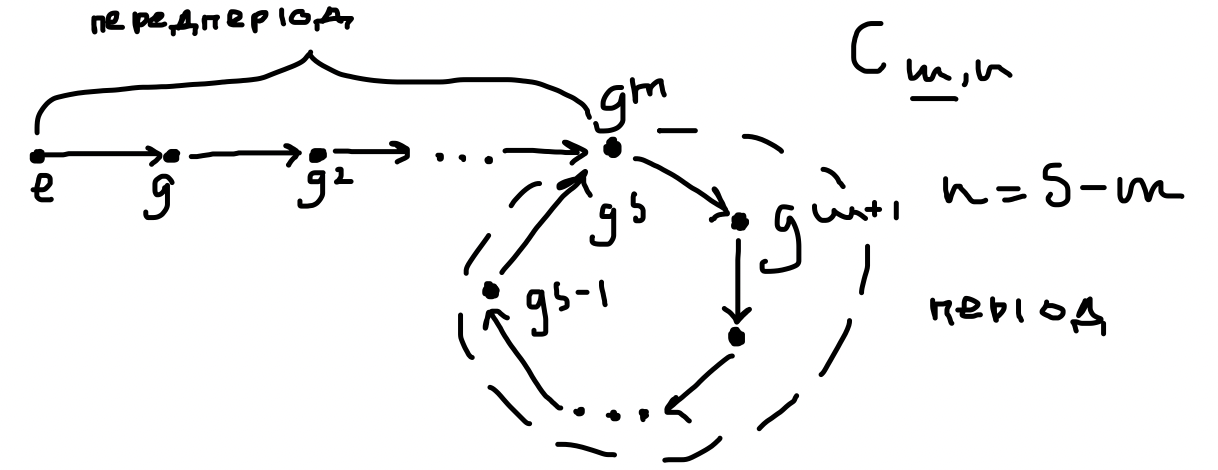
\includegraphics[width=6cm]{graph2.png}  
	\end{array}\begin{array}{l}
		\Mm=\langle g\rangle:\>g^k\mapsto k\\
		 \textrm{Нехай існує } \Mm=\langle g\rangle,\>|\Mm|<\infty\\\Rightarrow \exists \min g:\>g^s=g^m,\>m<s\\\langle2\rangle\in\mathbb{Z}_{20}\textrm{ за }\cdot \>\langle2\rangle=\{\overbrace{1,\>2}^{\textrm{передп.}},\overbrace{4,\>8,\>16,\>32}^{\textrm{цикл}}\}\sim C_{2,\>4}
	\end{array}$ 
\end{fact*}
\chapter{Лекція 2}
\section{Властивості елементів груп. Циклічні групи}
\begin{align*}
	\langle G,\>\cdot \rangle\> & \textrm{- замкненість}\\
	& \textrm{- асоціативність} \\
	& \textrm{- }\exists\textrm{ нейтральний елемент}\\
	& \textrm{- } \forall a\>\>\exists a^{-1}\>:\>a\cdot  a^{-1}=a^{-1}\cdot  a=e
\end{align*}
\begin{property*}$ $
	\begin{enumerate}
		\item Правило скорочення: $\\\forall a,\>x,\>y\in G:\tab ax=ay\Rightarrow x=y,\>xa=ya\Rightarrow x=y$
		\item $\forall a,\>b\in G:\tab$ $\begin{array}{c}
			ax=b\\ya=b
		\end{array}$ - мають єдиний розв'язок \begin{proof}$ $
			\begin{enumerate}\item $x=a^{-1}b:\tab ax=a(a^{-1}\cdot  b)=(a\cdot  a^{-1})b=e\cdot  b=b\Rightarrow$ - розв'язок
			\item Нехай $x_1,\>x_2$ - розв'язки $ax=b\tab \Rightarrow b=ax_1=ax_2\Rightarrow x_1=x_2$
			  \end{enumerate}
		\end{proof}
		\item \begin{prop*}$\forall a,\>b\in G$
			\begin{enumerate} 
				\item $e^{-1}=e$
				\item $(a^{-1})^{-1}=a$
				\item $(ab)^{-1}=b^{-1}a^{-1}$
				\item $\forall\in\mathbb{Z}:\>\>(a^{-1})^m=(a^m)^{-1}$
			\end{enumerate}
			\begin{proof}$ $
				\begin{itemize}
					\item [(c)] $(ab)^-1\cdot \underbrace{(ab)}_{x}=e,\>(ab)^{-1}\cdot  a\cdot  b\cdot  b^{-1}=(ab)^{-1}\cdot  a=e\cdot  b^{-1}=b^{-1},\>(ab)^{-1}=b^{-1}\cdot  a^{-1}$
				\end{itemize}
			\end{proof}
		\end{prop*}
		\item \begin{theorem} $\forall a\in G,\>\forall m,\>n\in\mathbb{Z}:$
			$$a^m\cdot  a^n=a^{m+n},\tab (a^m)^n=a^{mn}$$
			\begin{proof}$ $
				\begin{enumerate} 
					\item $\\$$\begin{array}{cl}
						a^m\cdot  a^n=a^{m+n}:& (1)\>m,\>n>0\textrm{ - доведено для }\forall\textrm{ моноїд}\\
						& (2)\>n,\>m<0\textrm{ - }a^m\cdot  a^n=(a^{-1})^{-m}(a^{-1})^{-n}\textrm{ - див. п. (1)}\\
						& (3)\begin{array}{ll} 
						m>0&a^ma^n=a^m(a^{-1})^t=\underbrace{aaa\dots a}_m\underbrace{a^{-1}a^{-1}\dots a^{-1}}_t\\
						n<0&m\geq t:\>=a^{m-t}=a^{m+n}\\
						t=-n<0&m<t:\>=(a^{-1})^{t-m}=a^{m-t}=a^{m+n}
						\end{array}\\
						&(4)\>m<0,\>n>0\textrm{ - аналогічно}
					\end{array}$
					\item $\\\begin{array}{ll}
						n\geq0:&(a^m)^n=a^m\cdot  a^m\cdot \dots\cdot  a^m=a^{mn}\\
						n<0:&(a^m)^n=((a^m)^{-1})^{-n}=((a^{-1})^m)^{-n}=(a^{-1})^{-mn}=a^{mn}
					\end{array}$
				\end{enumerate}
			\end{proof}
		\end{theorem}
	\end{enumerate}
\end{property*}
\begin{fact*}
	Циклічні групи $$G\textrm{ - циклічна}\Leftrightarrow\exists g:G=\langle g\rangle$$$$\Rightarrow\textrm{усі циклічні групи зводятся до }\langle\mathbb{Z},\>+\rangle$$$$\textrm{усі циклічні групи зводятся до }\langle \mathbb{Z}_m,\>
	+\rangle$$
\end{fact*}
\section{Порядок групи, порядок елементу групи. Підгрупи}
\begin{lemma}
	$$\langle G,\>\cdot \rangle,\>a\in G,\>\langle a\rangle\textrm{ - скінченна}\Rightarrow\langle a\rangle\textrm{ н містить передпорядку}$$ 
	\begin{proof}
		$\\\begin{array}{c}
			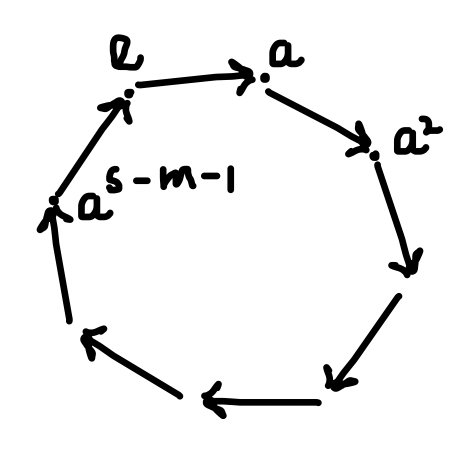
\includegraphics[width=3cm]{graph3}
		\end{array} \langle a\rangle$ - скінченна $\Rightarrow\begin{array}{l}
			\exists m,\>s:\>s>m>0.\\
			a^s=a^m\Rightarrow a^s\cdot (a^m)^{-1}=e,\>a^{s-m}=e.
		\end{array}$
	\end{proof}
\end{lemma}
\begin{definition}$\langle a\rangle$
	$$\textrm{ - орбітa елемента }a$$
\end{definition}
\begin{definition}$\ord G$
	$$\textrm{Порядок групи} = |G|$$
\end{definition}
\begin{definition}$\ord a$
	$$\textrm{Порядок елементу} = |\langle a\rangle|$$
	\begin{align*}
		\textrm{Якщо }\exists n\in\mathbb{N}:\>a^n=e,\textrm{ то }\ord a=\min\{n\>|\>a^n=e\},\>\textrm{ інакше }\ord a=\infty
	\end{align*}
\end{definition}
\begin{example}
	$\ord e=1,\tab \ord a=1\Leftrightarrow a=e$
\end{example}
\begin{example}
	$\langle\mathbb{Z},\>+\rangle:\>\ord0=1,\>\ord 1=\infty\\\langle\mathbb{Z}_4,\>+\rangle:\>\ord0=1,\>\ord1=4,\>\ord2=2$
\end{example}
\begin{lemma}
	\begin{align*}
		\textrm{Якщо }g\in G \textrm{ має скінченний порядок: }\ord g^u=n<\infty,\textrm{ то }g=e\Leftrightarrow u\>\vdots\>n
	\end{align*}
	\begin{proof}
		$\\$\textcircled{$\Leftarrow$} $u=k\cdot  n\Rightarrow g^u=(g^n)^k=e^k=e$$\\$\textcircled{$\Rightarrow$} Нехай $u\>\bar{\vdots}\>n\Rightarrow u=nq+r,\>0<r<n\\\tab e\cdot  g^u=(g^n)^q\cdot  g^r=e^q\cdot  g^r=g^r\Rightarrow n$ - не порядок $g$ - Упс!
	\end{proof}
\end{lemma}
\begin{definition}Підгрупа
	$$H\subseteq G\textrm{ - підгрупа }G\Leftrightarrow H\textrm{ - група}$$
	\begin{center}
		$\begin{array}{cl}
		\langle H,\>\cdot \rangle & - \textrm{ замкненість}\\
			 & - \textrm{ асоціативність}\\
			  & - \textrm{ наявність }e\\
			   & - \textrm{ наявність обернених}
	\end{array}$
	\end{center}	
\end{definition}
\begin{example}
	$\begin{array}{cl}
		\langle\mathbb{Z},\>+\rangle: & 2\mathbb{Z}\textrm{ - підгрупа}\\
		& n\mathbb{Z}=\{nm\>|\>m\in\mathbb{Z}\}\textrm{ - підгрупа}\\
		& 2\mathbb{Z}+1\textrm{ - не підгрупа (не замкнена)}\\
		& \mathbb{Z}_n\textrm{ - підгрупа}\mathbb{Z}
	\end{array}$
\end{example}
\begin{example}
	$\mathcal{S}L_n(\mathbb{R})\subseteq\mathcal{G}L_n(\mathbb{R}),\> \mathcal{S}L_n(\mathbb{R})=\{M\in\mathcal{G}L_n(\mathbb{R})\>|\>\det M=1\}$ - спеціальна підгрупа
\end{example}
Тривіальні підгрупи: $\{e\},\>G$, інші пігрупи - власні
\begin{prop*}
	$$H\subseteq G\textrm{ - }\Leftrightarrow\forall a,\>b\in H:\>\>a\cdot  b^{-1}\in H$$
\end{prop*}
\section{Класи суміжності, індекс підгрупи, теорема \\Лагранжа та наслідки з неї}
\begin{definition}Нехай $\langle G,\>\cdot \rangle$ - група, $H\subseteq G$ - підгупа 
	\begin{align*}
		\textrm{Елементи} g_1,\>g_2 - & \textrm{(ліво) конгуретні відносно} H: \begin{array}{l}
			g_1\equiv g_2(\mod n)\Leftrightarrow g_1^{-1}\cdot  g_2\in H\Leftrightarrow\\\Leftrightarrow\exists h\in H:g_2=g_1\cdot  h,\>g_1=g_2\cdot  h^{-1}
		\end{array}\\
		& \textrm{(право) конгурентні}\longrightarrow g_1\cdot  g_2^{-1}\in H\>\exists h\in H:\>g_2=h\cdot  g_1
	\end{align*}
\end{definition}
\begin{lemma}
	$$\equiv\mod H\leftarrow g_1\underset{H}{\sim}g_2\>(\textrm{відношення еквівалентності на }G)$$
\end{lemma}
$\begin{array}{cc}
	\textrm{лівий клас суміжності }g\in G: \>gH=\{gh\>|\>h\in H\} & \textrm{правий }:\>Hg=\{hg\>|\>h\in H\}	
\end{array}\\\Rightarrow G\bigcup\limits_{g\in G}gH$
\begin{prop*}усі класи суміжно рівнопотужні
	$$\forall g\in G\tab |gH|=|H|$$
	\begin{proof}
		Розглянемо відображення $fg:H\rightarrow gH\\\begin{array}{cl}
			fg(x)=g\cdot  x& - \textrm{ сюр'єктивне за побудовою } gH\\
			& - \textrm{ ін'єктивне: }x_1,\>x_2\in H\>\>fg(x_1)=fg(x_2),\>g\cdot  x_1=g\cdot  x_2,\>x_1=x_2 
		\end{array}\\\Rightarrow fg$ - бієкція $\Rightarrow|gH|=|H|$
	\end{proof}
\end{prop*}
\begin{definition}
	$$\textrm{Індекс пігрупи }H\textrm{ у групі }G:\>[G:H]=\textrm{кількість різник класів суміжності}$$
\end{definition}
$\\G\>- $ скінченна $\Rightarrow$ індекс скінченний\\
$G\>- $ не скінченна $\Rightarrow$ що завгодно
\begin{example}
	$[G:\{e\}]=|G|,\>[G:G]=1,\>\langle\mathbb{Z},\>+\rangle,\>H=n\mathbb{Z},\>[\mathbb{Z}:n\mathbb{Z}]=n$
\end{example}
\begin{theorem}[Lagrange]
	$$|G|=[G:H]\cdot|H|,\textrm{ якщо } G\textrm{ - скінченна}$$
	\begin{proof}
	$G=\bigcup\limits_{g}|gH|=\#$класiв сумижностi $\cdot\>|H|=[G:H]\cdot|H|$
\end{proof}
\end{theorem}
\begin{cons*}Нехай $|G|=n<\infty$
	\begin{enumerate}
		\item $\forall H$ - підгрупа: $n\>\vdots\>|H|$
		\item $\forall g\in G:\>n\>\vdots\>\ord g$ \begin{proof}
			$\ord g=|\langle g\rangle|,\>\langle g\rangle$ - підгрупа $G$
		\end{proof}
		\item $\forall g\in G:\>g^n=e$
		\item $\forall$ група простого порядку є циклічною\begin{proof}
			$|G|=p,\>p\geq 2$ - просте, $\exists g+e\Rightarrow\ord g\>|\>p,\>\ord g\neq1\Rightarrow\ord g=p\Rightarrow\\\Rightarrow|\langle g\rangle|=p\Rightarrow |\langle g\rangle|=G$
		\end{proof}
	\end{enumerate}
\end{cons*}
\begin{theorem}[Sylow]
	$$|G|=n,\>n\textrm{ - складене},\>p^\alpha\>|\>n,\>p\textrm{ - просте}\Rightarrow\exists H\subseteq\textrm{ - підгрупа, }|H|=p^\alpha$$
\end{theorem}
\begin{theorem}
	$$G\textrm{ - нециклічна скінченна абелева група},\>|G|=n\Rightarrow\exists u\>|\>n,\>u<n:\>\forall g\in G:\>g^u=e$$
\end{theorem}
Для $\langle\mathbb{Z}_m^*,\>\cdot \rangle$ число $u$ визначається функцією Кармайкла $\lambda(m)$
\chapter{Лекція 3}
\section{Властивості циклічних груп та їх елементів}
$G=\langle g\rangle=\{g^k\>|\>k\in\mathbb{Z}\}$\\
Генератор групи - довільне $g'\>\>G=\langle g'\rangle$
\begin{lemma}
	$$\forall H\subseteq G\textrm{ - підгрупа: }H\textrm{- циклічна}$$
	\begin{proof}
		$H$ - тривіальна - то очевидно ($H=\{e\}$ - ок, $H=G$ - за умови) \\
		$H$ - не тривіальна $\Rightarrow\exists g^k\in H,\>g^k\neq e\Rightarrow H:$ містить: $g^k:\>g^{-k}\Rightarrow\exists k>0:\>g^k\in H\\$ Нехай $s=\min\{k>o\>:\>g^k\in H\}\Rightarrow\langle g^k\rangle\subseteq H:\>?\subseteq \langle g^k\rangle\\\tab \forall t:\>g^t\in H\Rightarrow t\>\vdots\>s\\\tab $ Нехай $t\overline{\>\vdots\>},$ тоді $t=sq+r,\>0< t< s\Rightarrow g^r=g^{t-sq}=g^t\cdot  \left( g^s\right)^{-q}\in H$ - Упс!\\ $\tab\Rightarrow t\>\vdots\>s\Rightarrow g^t=\left(g^s\right)^q\subseteq\langle g^s\rangle\Rightarrow H\subseteq\langle g^s\rangle$
	\end{proof}
\end{lemma}
\begin{lemma}
	$$\ord g^k=\dfrac{n}{\gcd(n,\>k)},\textrm{ якщо}n=|G|<\infty$$
	\begin{proof}
		$\ord g^k=\min\{U>0\>:\>\left(g^k\right)^u=e\}\Rightarrow ku\>\vdots\>\ord g\Rightarrow ku\>\vdots\>n.$ Нехай $d=gcd(k,\>n)\\\tab k=k_1\cdot  d\tab k_1\cdot  d\cdot  u\>\vdots\>u\\\tab \gcd(k_1,\>n)=1\tab d\cdot u\>\vdots\>n\\\Rightarrow\min u=\dfrac nd\Rightarrow\ord g^k=\dfrac nd=\dfrac{n}{\gcd(n,\>k)}$
	\end{proof}
\end{lemma}
\begin{cons*}
	$$\textrm{Група } G\textrm{ містить }\varphi(n)\textrm{ генераторів}$$
\end{cons*}
\begin{lemma}
	$$\textrm{Якщо }d=\gcd(n,\>k),\textrm{ то }\langle g^k\rangle=\langle g^d\rangle$$
	\begin{proof}
		З одного боку, $k\>\vdots\>d\Rightarrow g^k=\left(g^d\right)^{\dots}\in\langle g^d\rangle\Rightarrow\langle g^k\rangle=\langle g^d\rangle$\\
		З іншого боку, $\ord g^k=|\langle g^k\rangle|=\dfrac nd,\>\ord g^d=|\langle g^d\rangle|=\dfrac n{\gcd(n,\>d)}=\dfrac nd\Rightarrow\\\Rightarrow|\langle g^k\rangle|=|\langle g^d\rangle|\Rightarrow \langle g^k\rangle=\langle g^d\rangle$
	\end{proof}
\end{lemma}
\begin{cons*}
	$$\textrm{Усі підгрупи }G\textrm{ однакового порядку співпадають}$$
	\begin{proof}
		$|\langle g^k\rangle|=|\langle g^M\rangle|\Rightarrow\ord g^k=\ord^M\Rightarrow\gcd(n,\>k)=\gcd(n,\>M)=d\\\Rightarrow\langle g^k\rangle=\langle g^d\rangle=\langle g^M\rangle$
	\end{proof}
\end{cons*}
\section{Стуруктура циклічних груп}
\begin{prop*}$G=\langle g\rangle,\>|G|=n<\infty$
	\begin{align*}
		\forall d\>|\>n:&-\textrm{існує єдинна підгрупа індексу } d\\
		&-\textrm{існує єдинна підгрупа порядку } d\\
		&-\textrm{існує рівно }\varphi(d) \textrm{ елементів порядку } d
	\end{align*}
	\begin{proof}$ $
		\begin{enumerate}
			\item $d\>|\>n\Rightarrow\langle g^d\rangle$ - підгрупа порядку $\dfrac nd\Rightarrow[G:\>\langle g^d\rangle=\dfrac n{n/d}-d$
			\item $d'=\dfrac nd\>:|>\langle g^{d'}\rangle$ - підгрупа порядку $d$
			\item елементи порядку $d$ - генератори $\langle g^{d'}\rangle\Rightarrow\exists\varphi(d)$ генераторів
		\end{enumerate}
		\begin{cons*}
			$$\sum\limits_{d\>|\>n}\varphi(d)=n$$
		\end{cons*}
	\end{proof}
\end{prop*}
\begin{center}
	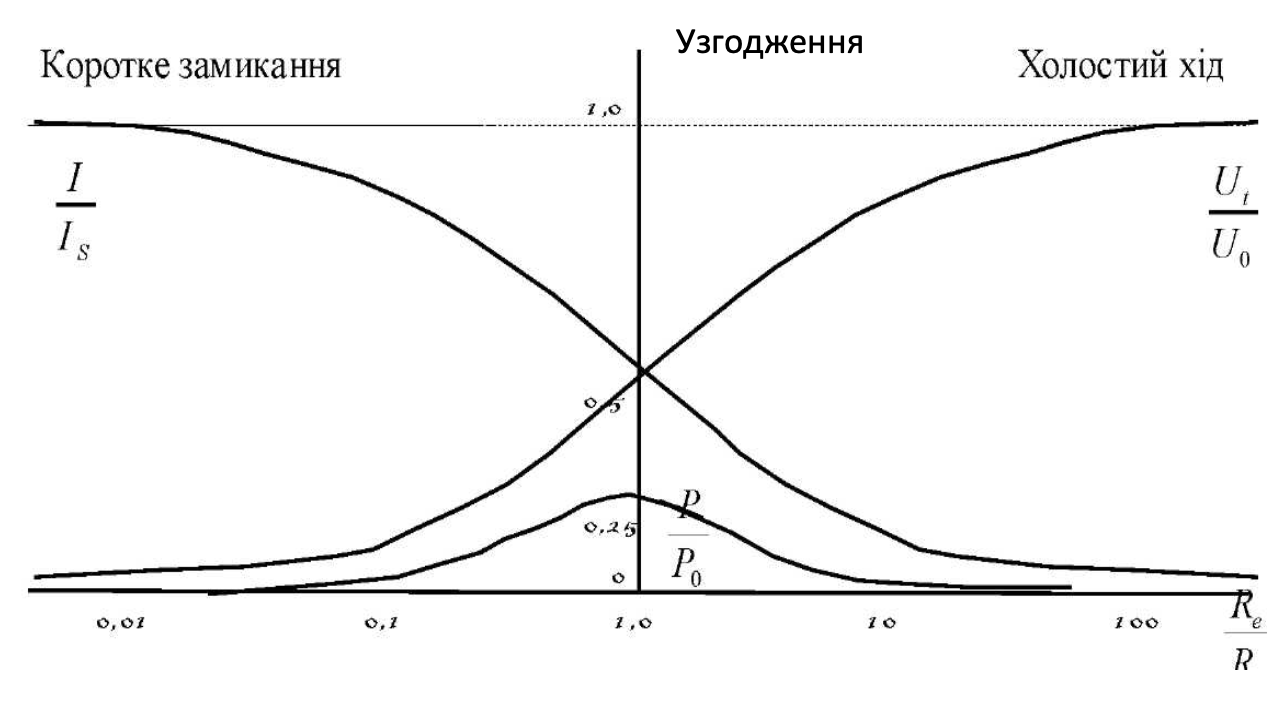
\includegraphics[width=16.5cm]{graph4}
\end{center}\newpage
\section{Нормальні підгрупи}
\begin{definition}$H\triangleleft G$
	$$H\subseteq G\textrm{ - нормальна}\Leftrightarrow\forall g\in G,\>\forall h\in H:\>\>ghg^{-1}\in H$$
\end{definition}

У абелевої групи усі підгрупи нормальні 
\begin{theorem}[equivalent conditions]
	\begin{align*}
		(1)\>\>& H\triangleleft G\\
		(2)\>\>& \forall g\in G:\>gHg^{-1}=H\\
		(3)\>\>& \forall g\in G:\>gH=Hg
	\end{align*}
	\begin{proof}
		\begin{align*}
			(1)\sim(2)&\textrm{ за означенням} :\>gHg^{-1}\subseteq H:\>H?\subseteq gHg^{-1}:\>\forall h\in H:\>\exists h'\in H:\>h=gHg^{-1}\\&\textrm{ Нехай } h'=g^{-1}\cdot h\cdot g\in H\textrm{ - з означення нормальності для } g^{-1}\\&\textrm{ Тоді } gh'g^{-1}=gg^{-1}hgg^{-1}=h\\(2)\sim(3)&\>gHg^{-1}=H\Leftrightarrow gH=Hg
		\end{align*}
	\end{proof}
\end{theorem}
\begin{wrapfigure}{r}{0.3\textwidth}
  \begin{center}
    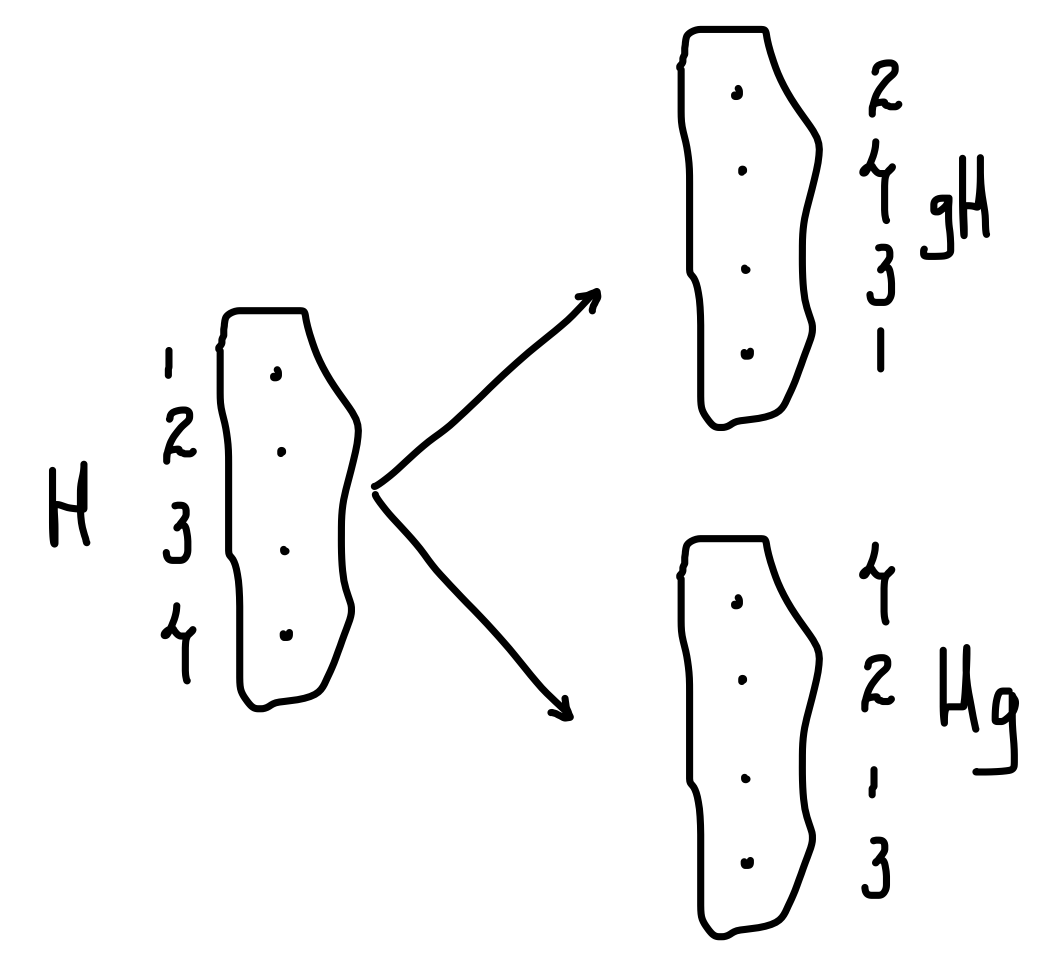
\includegraphics[width=0.2\textwidth]{graph5}
  \end{center}
\end{wrapfigure}
Введемо $G/ H=\{gh\>|\>g\in G\}$ - множина усіх класів суміжності.$\langle G,\>\cdot\rangle\Rightarrow\langle G/H,\>\cdot\rangle.\\(g_1H)\cdot(g_2H)=(g_1g_2)H\\fg(x)=gx\\hg(x)=xg$ \newblock
\section{Факор-групы}\newblock\\
\begin{theorem}
	$$\textrm{Якщо }H\triangleleft G,\textrm{ то }\langle G/H,\>\cdot\rangle\textrm{ - група (фактор-група)}$$
	\begin{proof}$\\$
		\begin{itemize}
			\item [$-$] замкненість - з побудови
			\item [$-$] успадкування з $\langle G,\>\cdot\rangle$
			\item [$-$] нейтральний елемент : $eH=H$
			\item [$-$] оберенений елемент : $\left(gH\right)^{-1}=\left(g^{-1}\right)H$\tab\tab де пастка?
			\item [] $\begin{array}{l}
				(\underset {\parallel}{g_1H})\cdot(\underset {\parallel}{g_2H})=(\underset {\cancel\parallel}{g_1g_2})H\\(a_1H)\cdot(a_2H)=(a_1a_2)H
			\end{array}$ - не факт, що $\cdot$ - операція
		\end{itemize}
		Треба довести, що $\left\{\begin{array}{l}
			a_1\equiv a_2\mod H\\
			b_1\equiv b_2\mod H
		\end{array} \right.\Rightarrow a_1b_1\equiv a_2b_2\mod H$
		\begin{itemize}
			\item [] $\begin{array}{lll}
				\exists h_{a_1},\>h_{a_2}\in H: &a_1=h_a\cdot a_2 & \Rightarrow a_1b_1=h_1\cdot a_2\cdot h_b\cdot b_2\\&&\textrm{Але: }H\textrm{ - нормальна підгрупа}\\&&\Rightarrow a_2H=Ha_2\Rightarrow\exists h_c:\>a_2h_b=h_ca_2\\&&\Rightarrow a_1b_1=h_ah_c\cdot a_2b_2\Rightarrow a_1b_!\equiv a_1b_1\equiv a_2b_2\mod H
			\end{array}$
		\end{itemize}	
	\end{proof}
	\textcircled{$\Rightarrow$} $G/H$ - фактор-група. $|G/H|=[G:H]=\dfrac{|G|}{|H|},$ якщо $|G|<\infty$
\end{theorem}
\section{Морфізми алгебраїчних структур}
\begin{definition}$\langle S,\>\cdot\rangle,\>\langle A,\>\times\rangle$ - алгебраїчні структури
	\begin{align*}
		\textrm{Гомоморфізм:}\tab & f:S\to A,\>\forall a,\>b\in S:\>f(a\cdot b)=f(a)\times f(b)\\\textrm{Мономорфізм:}\tab  & \textrm{ін'єктивний гомоморфізм}\\
		\textrm{Епіморфізм:}\tab & \textrm{сюр'єктивний гомоморфізм}\\
		\textrm{Ізооморфізм:}\tab & \textrm{бієктивний гомоморфізм}\\&S\sim A\textrm{ ізоморфні структури}
	\end{align*}
\end{definition}
\textcolor{red}{\scalerel*{!}{\bigg)}} З точки зору абстрактної алгебри ізоморфні структури співпадають: \\\tab\tab властивості, які випливають з аксіом, співпадають:\\\tab\tab  - існує єдина група порядку 2 (з точністю до ізоморфізму)\\\tab\tab  - існує єдина нескінченна циклічна група (з точністю до ізоморфізму)
\begin{definition}
	\begin{align*}
		\textrm{Розділяемо } & \textrm{ гомоморфізм моноїдів та груп. }\\
		\textrm{Ендоморфізм: } & \textrm{ гоморфізм алгеброїчною структури саму на себе.}\\
		\textrm{Автоморфізм: } & \textrm{ бієктивний ендоморфізм.}
	\end{align*}
\end{definition}
\begin{fact*}$\forall S\textrm{ - напівгрупа}$
	$$\textrm{множина її автоморфізмів утворює группу }\langle Aut(S),\>\circ\rangle$$
\end{fact*}
Поняття нормальності підгрупи пов'язане з внутрішнім автоморфізмами \\\tab $\varphi_a(x)=a\times a^{-1}$\newpage
\begin{example}
	$\langle\mathbb{R},\>+\rangle,\>\langle\mathbb{R}^+,\>\cdot\rangle\tab \mathbb{R}^+=\{x\in\mathbb{R}\>:\>x>0\}\\ f(x)=e^x:\>f(x+y)=e^{x+y}=e^x\cdot e^y=f(x)\cdot f(y)\\ f^{-1}(x)=\ln x\Rightarrow f$ - ізоморфізм
\end{example}
\begin{example}
	$f(a)=a\mod n:\tab$ гомоморфізм $\langle\mathbb{Z},\>+\rangle$ на $\langle\mathbb{Z}_n,\>+\rangle,\>\langle\mathbb{Z},\>\cdot\rangle$ на $\langle\mathbb{Z}_n,\>\cdot\rangle$\\ сюр'єктивне $\Rightarrow$ епіморфізм
\end{example}
\begin{example}
	\begin{align*}
		\det:\>Mat_{n\times n}(\mathbb{R})\to\mathbb{R}&\textrm{ - гомоморфізм за множенням}\\ \det\left[\begin{array}{ll@{}}
a &0\\
0 & \ddots 
\end{array}\right] = a&\textrm{ - епіморфізм}\\\det:\>Mat_{n\times n}(\mathbb{R})\to\mathbb{C}&\textrm{ - не епіморфізм}
	\end{align*}
\end{example}
\chapter{Лекція 4}
\section{Tеорема про гомоморфізм груп}

\begin{lemma}$\langle G,\>\cdot\rangle,\>\langle H,\>\times\rangle,\>f:G\to H$ гомоморфізм груп
	\begin{align*}
		(1)&\>f(e_G)=e_H\\
		(2)&\>f(a_G^{-1})=(f(a_H))^{-1}
	\end{align*}
	\begin{proof}$\\$
		\begin{itemize}
			\item [(1)] $\forall a\in G:\>f(a\cdot e_G)=f(a)\times f(e_H)=e_H=f(e_G)$
		\end{itemize}
	\end{proof}
\end{lemma}
\begin{definition}Ядро гомоморфізму $$\ker f=f^{-1}(e_H)=\{a\in G\>:\>f(a)=e_h\}$$ 
\end{definition}
\begin{definition}Образ гомоморфізму $$\im f=f(G)=\{b\in H\>|\>\exists a\in G:\>f(a)=b\}$$
	
\end{definition}
\begin{example}
	$f(a)=a\mod n,\tab f:\mathbb{Z}\to\mathbb{Z}_n\\\Rightarrow\ker f=n\mathbb{Z},\>\im f=\mathbb{Z}_n$
\end{example}
\begin{example}
	$\det:\mathcal{G}L_n(\mathbb{R})\to\mathbb{R}\\\ker(\det)=\{A\>|\>\det A=1\}=\mathcal{S}L_n(\mathbb{R}),\>\im(\det)=\mathbb{R}\backslash\{0\}$
\end{example}
\begin{theorem}[group homomorphism]$\\\tab\langle G,\>\cdot\rangle,\>\langle H,\>\times\rangle,\>f:G\to H$ гомоморфізм груп
	\begin{align*}
		(1)&\>\ker f\textrm{нормальна підгрупа }G\\
		(2)&\>G/\ker f\sim\im f
	\end{align*}\newpage
	\begin{proof}
		$\\$\begin{itemize}
			\item [(1)] $?\>\forall g\in G,\>\forall a\in\ker f:\>gag^{-1}\in\ker f:\tab f(gag^{-1})=f(g)\times f(a)\times f(g^{-1})=f(g)\times e_H\times(f(g))^{-1}=f(g)\times(f(g))^{-1}=e_H\Rightarrow gag^{-1}\in\ker f$
			\item [(2)] $K=\ker f:$ побудуємо ізоморфізм $\psi:G/K\to\im f,\>\psi(gK):=f(g)\\$
				$\\\begin{array}{lll}
					(a)&\textrm{коректність: } & g_1\equiv g_2(\mod K)\Leftrightarrow\psi(g_1)=\psi(g_2)\>(\Rightarrow f(g_1)=f(g_2))\\&&\exists a\in K:\>g_1=a\cdot g_2,\> \psi(g_1k)=f(g_1)=f(a\cdot g_2)=\\&&=f(a)\times f(g_2)=e_H\times f(g_2)	=f(g_2)
				\end{array}\\\\\begin{array}{lll}
					(b)&\textrm{гомоморфізм - з побудови: }&\psi(g_1k\cdot g_2k)=g(g_1g_2)=f(g_1)\times f(g_2)=\\&&=\psi(g_1k)\times\psi(g_2k)
				\end{array}\\\\\begin{array}{lll}
					(c)&\textrm{сюр'єктивність - з означення }\im t 
				\end{array}\\\\\begin{array}{lll}
					(d)&\textrm{ін'єктивність: }&\psi(g_1k)=\psi(g_2k)\Rightarrow f(g_1)=f(g_2)\Rightarrow f(g_1)\times (f(g))^{-1}=\\&&=e_H\Rightarrow f(g_1\cdot g_2^{-1})=e_H,\>g_1\cdot g_2^{-1}\in K\Rightarrow g_1=g_2(\mod K)
				\end{array}\\\Rightarrow\psi$ - ізоморфізм 
		\end{itemize}
	\end{proof}
\end{theorem}
\begin{prop*}
	\begin{align*}
		\textrm{Якщо }H\triangleleft G\textrm{, то відображення }&\varphi:G\to G/H\textrm{ - гомоморфізм}\\&\varphi(g):=gH\tab \ker\varphi =H
	\end{align*}
\end{prop*}
\section{Кільця}
$\langle A,\>+,\>\cdot\rangle,$ + = "додавання", $\cdot$ = "множення"  
\begin{definition}$\langle\mathcal{R},\>+,\>\cdot\rangle$
	\begin{align*}
		\textrm{ - кільце}\tab&(1)\>\langle\mathcal{R},\>+\rangle\textrm{ - абелева група}\\&(2)\>\langle\mathcal{R},\>\cdot\rangle\textrm{ - напівгрупа}\\&(3)\>\textrm{дистрибутивність: }\forall a,\>b\in\mathbb{R}:&(a+b)\cdot c=a\cdot c+b\cdot c\\&&c\cdot(a+b)=c\cdot a+c\cdot bx
	\end{align*}
\end{definition}
Якщо $\mathcal{R}=\{r\}$, то - тривіальне кільце - нудне та нецікаве $\Rightarrow|\mathcal{R}|\geq2$
\begin{example}
	$\mathbb{R},\>\mathbb{C},\>\mathbb{Q}$ - кільця за $+,\>\cdot$
\end{example}
\begin{example}
	кільце лишків $|\mathbb{Z}_n|\>(+\mod,\>\cdot\mod)$
\end{example}
\begin{example}
	кільце матриць $Mat_{n\times m(\mathbb{R})}$
\end{example}
\begin{example}
	кільце поліномів $R[x]=\left\{\displaystyle\sum_{k=0}^na_kx^k\>|\>a_k\in\mathbb{R}\right\}$
\end{example}
\begin{definition}
	$$\mathcal{R}^+\equiv\langle\mathcal{R},\>+\rangle\textrm{ - адетивна група кільця }\mathcal{R}$$
	$$\textrm{Нуль кільця - нейтральний елемент - }\mathcal{O}\>(\mathcal{O}_{\mathcal{R}})$$
	$$\textrm{обернене за додаванням}: -a$$
	$$\forall m\in\mathbb{Z}:\>ma=\left\{\begin{array}{l}
		a+a+\dots+a,\>m>0\\
		(-a)+(-a)+\dots+(-a),\>m<0
	\end{array} \right.$$
\end{definition}
\begin{lemma}
	\begin{align*}
		\textrm{у довільному кільці }\mathcal{R}:\tab&(1)\>\forall a\in\mathcal{R}:&0\cdot a=a\cdot0=0\\&(2)\>\forall a,\>b\in\mathcal{R}:&(-a)\cdot b=a\cdot (-b)=-(a\cdot b)
	\end{align*}
	\begin{proof}
		$\\\>(1)\>0=0+0\Rightarrow0\cdot a=(0+0)\cdot a=0\cdot a+0\cdot a\\\textrm{ }\>\>\>\>\>0=0\cdot a$ аналогічно $a\cdot0=0$
	\end{proof}
\end{lemma}
\section{Напівкільця}
\begin{definition}$\langle\mathcal{S},\>+,\>\cdot\rangle$
	\begin{align*}
		\textrm{- напівкільце}\tab&(1)\>\langle\mathcal{S},\>+\rangle\textrm{ - комутативний мноїд}\\&(2)\>\langle\mathcal{S},\>\cdot\rangle\textrm{ - напівгрупа}\\&(3)\>\textrm{дистрибутивність}\\&(4)\>\textrm{мультиплікативність нуля}:&\forall a\in\mathcal{S}:\>0\cdot a=a\cdot0=0
	\end{align*}
\end{definition}
\begin{example}
	$\mathbb{N}_0$ - напівкільце за $+,\>\cdot$ (нема оберненого елмента за додаванням)
\end{example}
\begin{example}
	$\langle \{Q\},\>\oplus,\>\&\rangle$ - булеве напівкільце (нема оберненого елмента за множенням)
\end{example}
\section{Класи кілець, підкільця, ідеали}
\textbf{Типи кілець:}
\begin{enumerate}
	\item кільце з одиницею: $\langle \mathcal{R},\>\cdot \rangle$ - моноїд, нейтральний елмент - $1\>(1_\mathcal{R})$ - одиниця за множенням. $\mathcal{R}$ - нетривіальне $\Rightarrow0\neq1$
	\item комутативне кільце: $\cdot$ - комутативне
	\item кільце без дільника нуля: \\$a\cdot b=0,\>a\neq0,\>b\neq0\Rightarrow a$ - лівий, $b$ - правий дільники нуля\\$\Rightarrow\forall a,\>b\in\mathcal{R}:\>a\cdot b\Rightarrow(a=)\lor(b=0)$ 
	\item область цілісності (цілісне кільце) (integral domain) - комутативне кільце за одиниею і без дільників нуля\\$$\mathcal{R}\textrm{ - цілісне кільце}\Leftrightarrow\forall a\neq0,\>b,\>c\in\mathcal{R}:\>a\cdot b=a\cdot c\Rightarrow b=c$$
\end{enumerate}
\begin{definition}$\langle\mathcal{F},\>+,\>\cdot\rangle$
	$$\textrm{Поле - кільце, у якому }\langle\mathcal{F}\backslash\{0\},\>\cdot\rangle\textrm{ - абелева група}$$
\end{definition}
\begin{fact*}
	$$\textrm{Поле - цілісне кільце, скінчене цілісне кільце - поле}$$
\end{fact*}
\begin{example}
	$\mathbb{R},\>\mathbb{C},\>\mathbb{Q}$ - поля
\end{example}
\begin{example}
	$\mathbb{Z}$ - цілісне кільце, $2\mathbb{Z}$ - комутативне кільце без одиниці 
\end{example}
\begin{example}
	$\mathbb{Z}_n$ - комутативне кільце з одиницею. $n$ - просте $\Rightarrow\mathbb{Z}_n$ - поле, \\$n$ - складне $\Rightarrow$ є дільники нуля
\end{example}
\begin{example}
	$Mat_{n\times m}(\mathbb{R})$ - некомутативне кільце з одиницею
\end{example}
\begin{definition}
	$$a^{-1}\textrm{ - оборотний, якщо }\exists a^{-1}\in\mathcal{R}:\>a\cdot a^{-1}=a^{-1}\cdot a=1$$
	$$\mathcal{R}^*\textrm{ - множина усіх оборотних елментів }\mathcal{R}$$
\end{definition}
\begin{lemma}
	$$\langle\mathcal{R}^*,\>\cdot\rangle\textrm{ - група}$$
\end{lemma}
\begin{definition}
	$$\textrm{Підкільце }\mathcal{R}'\subseteq\mathcal{R}.\>\langle\mathcal{R}',\>+,\>\cdot\rangle\textrm{ - кільце}$$
\end{definition}
\begin{lemma}[subring criterion]
	\begin{align*}
		\mathcal{R}'\subseteq\mathcal{R}\tab\Leftrightarrow\tab&(1)\>1_\mathcal{R}\in\mathcal{R}'\\&(2)\>\forall x,\>y\in\mathcal{R}':&x-y\in\mathcal{R}'\\&&x\cdot y\in\mathcal{R}'
	\end{align*}
\end{lemma}
\begin{definition}
	\begin{align*}
		\textrm{Ідеал }\mathcal{I}\subseteq\mathcal{R}\tab\Leftrightarrow\tab&(1)\>\mathcal{I}\textrm{ - підкільце}\\&(2)\>\forall a\in\mathcal{I},\>\forall r\in\mathcal{R}:&a\cdot r\in\mathcal{I},\>r\cdot a\in\mathcal{I}
	\end{align*}
\end{definition}
\begin{example}
	$\mathbb{Z}$ - підкільце у $\mathcal{R}$, але не ідеал
\end{example}
\begin{example}
	$2\mathbb{Z},\>n\mathbb{Z}$ - ідеали у $\mathbb{Z}$
\end{example}


















\begin{appendices}
\appendixpage
\noappendicestocpagenum
\addappheadtotoc

\chapter[A]{Appendix}
\section{Подільність многочленів}
$1+x+x^2+x^3+\dots+x^{n-1}=S(x)\\ 1+x(1+x+x^2+\dots+x^{n-2}=1+x(s(x)-x^{n-1}=S(x)$
$$x^{n-1}=(X-1)(x^{n-1}+x^{n-2}+\dots+x+1)$$
\section{Наслідок з подільності(теорема Безу)}
$x\to\dfrac{x}{y}:\tab \dfrac{x^n}{y^n}-1=(\dfrac xy-1)(\dfrac{x^{n-1}}{y^{n-1}}+\dfrac{x^{n-2}}{y^{n-2}}+\dfrac xy+1)\tab \big|\>x\tab \cdot y^n$
$$x^n-y^n=(x-y)(x^{n-1}+	x^{n-2}y+x^{n-3}y^2+\dots+xy^{n-2}+y^{n-1}$$
$$\Rightarrow(x^n-y^n)\>\vdots\>(x-y)$$
Поліном: $p(x)=a_nx^n+a_{n-1}x^{n-1}+\dots+a_1x+a_0,\>a_n\in\mathbb{R},\>a_n\neq0,\>\deg p=n\\\tab p(x)-p(y)=a_n(x^n-y^n)+a_{n-1}(x^{n-1}-y^{n-1})+\dots+a_1(x-y)+a_0\cdot0\\\tab p(x)-p(y)\>\vdots\>(x-y),\> p(x)-p(y)=(x-y)\cdot Q(x,\>y),\>Q(x,\>y)_{\textrm{ - поліном від } x,\>y}$
\begin{theorem*}[Безу]
	$$p(x)\textrm{ - поліном},\forall\>\alpha\textrm{ - число}\Rightarrow p(x)-p(\alpha)\>\vdots\>(x-\alpha)$$
	\centering або
	$$\forall\>\alpha\textrm{ - число}\>\exists q(x):\>p(x)=(x-\alpha)\cdot q(x)+p(\alpha),\>\deg q=\deg p-1$$
\end{theorem*}
\section{Наслідок з теореми Безу}
\begin{enumerate}
	\item якщо $\alpha$ - корінь $p(x),$ то $p(x)\>\vdots\>(x-\alpha)\\p(\alpha)=0\Rightarrow p(x)=(x-\alpha)\cdot q(x)+p(\alpha)=(x-\alpha)\cdot q(x)$
	\item якщо $\alpha_1,\>\alpha_2,\dots,\alpha_n\in\mathbb{C}$ - усі корені з урахуванням кратності, то \\ $p(x)=a_n(x-\alpha_1)(x-\alpha_2)\dots(x-\alpha_n)$
\end{enumerate}
\section{Теорема Вієта}
$\tab x^n:\>a_n=a_n\\\tab x^{n-1}:\>a_{n-1}=a_n(-\alpha_1-\alpha_2-\dots-\alpha_n)\Rightarrow\alpha_1+\alpha_2+\dots+\alpha_n=-\dfrac{a_{n-1}}{a_n}\\p(x)=a_3x^3+a_2x^2+a_1x+a_0=a_3(x-\alpha_1)(x-\alpha_2)(x-\alpha_3)=a_3(x^3-\alpha_1x^2-\\-\alpha_2x^2-\alpha_3x^2\alpha_1\alpha_2x+\alpha_1\alpha_3x+\alpha_2\alpha_3x-\alpha_1\alpha_2\alpha_3)\\\Rightarrow\begin{array}{rl}
	x^3:&a_3=a_3\\
	x^2:&a_2=a_3(-\alpha_1-\alpha_2-\alpha_3)\\
	x:&a_1=a_3(\alpha_1\alpha+\alpha_1\alpha_3+\alpha_2\alpha_3)\\
	x^0=1:&a_0=a_3(-\alpha_1\alpha_2\alpha_3)
\end{array}\begin{array}{c}
	x^k: a_k=a_n\cdot(-1)^{n-k}\sum\alpha_{i_1}\alpha_{i_2}\dots\alpha_{i_k}\\1\leq i_1<i_2<\dots<i_n\leq n
\end{array}\\
\tab\Rightarrow\alpha_1+\alpha_2+\dots+\alpha_n=-\dfrac{a_{n-1}}{a_n},\tab\alpha_1\alpha_2\dots\alpha_n=(-1)^n\cdot\dfrac{a_0}{a_n}$
\section{Схема Горнера}
$\tab p(x)=a_nx^n+a_{n-1}x^{n-1}+\dots+a_1x+a_0\\
\tab q(x)=b_nx^n+b_{n-1}x^{n-1}+\dots+b_1x+b_0\\
p(x)=(x-\alpha)\cdot q(x)+p(\alpha)=(x-\alpha)(b_{n-1}x^{n-1}+\dots+b_1x+b_0)+p(\alpha)=\\\begin{array}{lllllll}
	=b_{n-1}\cdot x^{n} & +b_{n-2}\cdot x^{n-1} & +b_{n-3}\cdot x^{n-2} & +\dots & +b_1\cdot x^2 & +b_0\cdot x & \\
	 & -\alpha b_{n-1}x^{n-1} & -\alpha b_{n-2}x^{n-2} & -\dots & -\alpha b_2x^2 & -\alpha b_1x & -\alpha b_0 +p(\alpha)= 
\end{array}\\=a_n\cdot x^n+a_{n-1}\cdot x^{n-1}+\dots+a_1x+a_0\\\Rightarrow\begin{array}{l}
	a_n=b_{n-1}\\a_{n-1}=b_{n-2}-\alpha\cdot b_{n-1}\\a_{n-2}=b_{n-3}-\alpha\cdot b_{n-2}\\\tab\vdots\\a_1=b_0-\alpha b_1\\a_0=p(\alpha)-\alpha b_0
\end{array}\Rightarrow\begin{array}{l}
	b_{n-1}=a_n\\b_{n-2}a_{n-1}+\alpha\cdot b_{n-1}\\b_{n-3}=a_{n-2}+\alpha\cdot b_{n-2}\\\tab\vdots\\b_0=a_1+\alpha b_1\\p(\alpha)=a_0+\alpha b_0
\end{array}$
\begin{center}
\begin{table}[!htp]
\centering
\begin{tabular}{c|c|c|c|c|c|c|c}
           & $a_n$     & $a_{n-1}$ & $a_{n-2}$ & $\dots$ & $a_{n}$ & $a_1$         & $a_0$       \\ \hline
$\alpha$   & $b_{n-1}$ & $b_{n-2}$ & $b_{n-3}$ & $\dots$ & $b_1$   & $b_0$         & $p(\alpha)$ \\ \hline
$\alpha_2$ & $c_{n-2}$ & $c_{n-3}$ & $c_{n-4}$ & $\dots$ & $c_0$   & $q(\alpha_2)$ &            
\end{tabular}
\end{table}
\end{center}
$\slash*\\$\tab Задача схеми Горнера - поділити многочлен на $(x-\alpha)$, не обчислюючи усі степені $\alpha$.
Ефективніший за ділення у стовпчик - простий (лише 1 "+" та 1 "$x$" на одну клітинку) та швидкий (один цикл for + перекладання з одного масиву у інший)\begin{flushright}
$*\slash$
\end{flushright}
\section{Ланцюгові дроби}
$\alpha\in\mathbb{R}:\>\>\alpha=a_1+a_0,\>a_\in\mathbb{Z},\>0\leq\alpha_1<1\\
\alpha=a_1+\dfrac{1}{\dfrac{1}{\alpha_1}}=a_1+\dfrac{1}{\dfrac{a_2}{\alpha_2}}=a_1+\dfrac{1}{a_2+\dfrac{1}{\dfrac{1}{\alpha_2}}}=a_1+\dfrac{1}{a_2+\dfrac{1}{a_3+\alpha_3}}=\dots\\$
Ланцюговий дріб $\alpha$ - представлення $\alpha$ у вигляді $a_1+\dfrac{1}{a_2+\dfrac{1}{a_3+\alpha_3}}\>:\>\alpha=[a_1;\>a_2,\>a_3,\>a_4,\dots],\\\>a_1\in\mathbb{Z},\>a_1\in\mathbb{N}_0$
\section{Чим більше знаємо дробів - тим точніше $\alpha$}
$$\alpha=a_1+\dfrac{1}{a_2+\dfrac{1}{a_3+\dfrac{1}{a_4+\dfrac{1}{a_5+\dots}}}}$$
\section{Кожен скінченний дріб описує одне раціональне число}
\begin{prop*} $$\alpha\in\mathbb{Q},\>\alpha=\dfrac mn \Leftrightarrow\alpha \textrm{ має скінченний ланцюговий дріб}$$ 
	\begin{proof}$ $
		\begin{itemize}
			\item [$\Leftarrow$] $[a_1;\>a_2,\>a_3,\dots,\>a_t]=a_1+$
\begin{tabular}{ccccc}
\multicolumn{2}{c}{1}      &            &                 &       \\ \cline{1-2}
$a_2+$    & \multicolumn{2}{c}{1}       &                 &       \\ \cline{2-3}
          & $a_3+$         & \multicolumn{2}{c}{1}        &       \\ \cline{3-4}
          &                & \multicolumn{2}{c}{$\ddots$} &       \\
          &                &            & $a_{t-1}+$      & 1     \\ \cline{5-5} 
          &                &            &                 & $a_t$
\end{tabular} $=\dots=\dfrac mn$
			\item [$\Rightarrow$] (Алгоритм Евкліда!) $\\\alpha=\dfrac mn =\dfrac{r_0}{r_1}=\dfrac{r_1q_1+r_2}{r_1}=q_1+\dfrac{r_2}{r_1}=q_1+\dfrac1{\dfrac{r_1}{r_2}}=q_1+\dfrac1{q_2+\dfrac{r_3}{r_2}}=\dots=\\=q_1+$\begin{tabular}{ccccc}
\multicolumn{2}{c}{1}      &            &                 &       \\ \cline{1-2}
$q_2+$    & \multicolumn{2}{c}{1}       &                 &       \\ \cline{2-3}
          & $q_3+$         & \multicolumn{2}{c}{1}        &       \\ \cline{3-4}
          &                & \multicolumn{2}{c}{$\ddots$} &       \\
          &                &            & $+$      & 1     \\ \cline{5-5} 
          &                &            &                 & $q_n$
\end{tabular} $\Rightarrow\alpha=[q_1;\>q_2,\>q_3,\dots,\>q_n]$
		\end{itemize}
	\end{proof}
\end{prop*}
$\slash*\\$\begin{itemize}
	\item [$\Leftarrow$]Усі $a_i$ - цілі, невід'ємні (нулі лише для ірраціональних випадків), крім $а_1$ - воно може бути від'ємним, цілим. (тому ми його відділяємо;) 
	\item [$\Rightarrow$] Алгоритм Евкліда скінченний, тому фокус такий.
\end{itemize}
\begin{flushright}
$*\slash$
\end{flushright}
\section{Наближення числа $\pi$}
$\dfrac{22}7\approx\pi:\tab $
\begin{tabular}{ll|l|llll}
\cline{3-3}
22 & = & 3 & $\cdot$ & 7 & + & 1 \\
7  & = & 7 & $\cdot$ & 1 & + & 0 \\ \cline{3-3}
\end{tabular}$\tab\Rightarrow\tab \dfrac{22}7=3+\dfrac17\\\\$
$\dfrac{25}7:\tab $
\begin{tabular}{ll|l|llll}
\cline{3-3}
25 & = & 3 & $\cdot$ & 7 & + & 4 \\
7  & = & 1 & $\cdot$ & 4 & + & 3 \\
4  & = & 1 & $\cdot$ & 3 & + & 1 \\
3  & = & 3 & $\cdot$ & 1 & + & 0 \\ \cline{3-3}
\end{tabular}$\tab\Rightarrow\tab\begin{array}{c}
	\dfrac {25}7=3+\dfrac1{1+\dfrac1{1+\dfrac13}}=3+\dfrac1{1+\dfrac43}=\\=3+\dfrac1{\dfrac74}=\dfrac{25}7
\end{array}$











\end{appendices}





\end{document}